\documentclass[a4paper, 11pt, french]{article}

\usepackage[french]{babel}
\usepackage[T1]{fontenc}
\usepackage[utf8]{inputenc}
\usepackage{numprint}

\usepackage{algorithmicx}
\usepackage{algorithm}
\usepackage{algpseudocode}
\usepackage{float}
\usepackage{mathtools}
\usepackage{amssymb}
\usepackage{amsthm}
\usepackage{amsmath}
\usepackage{amsfonts}
\usepackage{lscape}
\usepackage{wrapfig}
\usepackage{rotating}

\usepackage{fullpage}
\usepackage{hyperref}
\usepackage{nameref}
\usepackage{xcolor}
\usepackage{graphicx}
\usepackage{enumitem}
\usepackage{listings}
\usepackage{xspace}

\usepackage{tikz}

\graphicspath{{images/}}

% Traductions
\makeatletter
\renewcommand{\ALG@name}{Algorithme}
\renewcommand{\listalgorithmname}{Liste des \ALG@name s}
\renewcommand{\algorithmicrequire}{\textbf{Entrée :}} 
\renewcommand{\algorithmicensure}{\textbf{Sortie :}} 
\renewcommand{\algorithmicend}{\textbf{fin}}
\renewcommand{\algorithmicif}{\textbf{si}}
\renewcommand{\algorithmicthen}{\textbf{alors}}
\renewcommand{\algorithmicelse}{\textbf{sinon}}
\renewcommand{\algorithmicfor}{\textbf{pour}}
\renewcommand{\algorithmicforall}{\textbf{pour chaque}}
\renewcommand{\algorithmicdo}{\textbf{faire}}
\renewcommand{\algorithmicwhile}{\textbf{tant que}}
\renewcommand{\algorithmicloop}{\textbf{boucle}}
\renewcommand{\algorithmicrepeat}{\textbf{répéter}}
\renewcommand{\algorithmicuntil}{\textbf{jusqu'à ce que}}
\renewcommand{\algorithmicreturn}{\textbf{retourner}}
\newcommand{\new}{\textbf{nouveau}\xspace}
\makeatother
\newcommand{\entree}[1]{\Require #1} 
\newcommand{\sortie}[1]{\Ensure #1}

% Références vers des algo
\newcommand{\algorithmautorefname}{algorithme}
\newcommand{\definitionautorefname}{définition}

% Définitions mathématiques
\theoremstyle{definition}
\newtheorem{definition}{Définition}

\hypersetup{colorlinks=true,breaklinks=true,urlcolor=cyan,linkcolor=gray,citecolor=green}

% Pour faire do-while
\algdef{SE}[DOWHILE]{Do}{DoWhile}{\algorithmicdo}[1]{\algorithmicwhile\ #1}%

% Pour être plus lisible
\newcommand{\mean}[1]{\overline{#1}}

\def\sun{s_{1}}
\def\sde{s_{2}}
\def\ademi{_{\frac{\alpha}{2}}}

\definecolor{darkblue}{rgb}{0.0,0.0,0.6}
\definecolor{darkred}{rgb}{0.3,0.0,0.0}

\lstset{%
    breaklines=true,
        columns=fullflexible,
            showstringspaces=false
}

\title{Résumé-explications de Simulation}
\author{Virgile Brouillard\and Jonathan Joertz\and Dorian Labeeuw\and Gaëtan Staquet}

\begin{document}

\maketitle

\tableofcontents

\section{Lois discrètes}
\begin{figure}[H]
    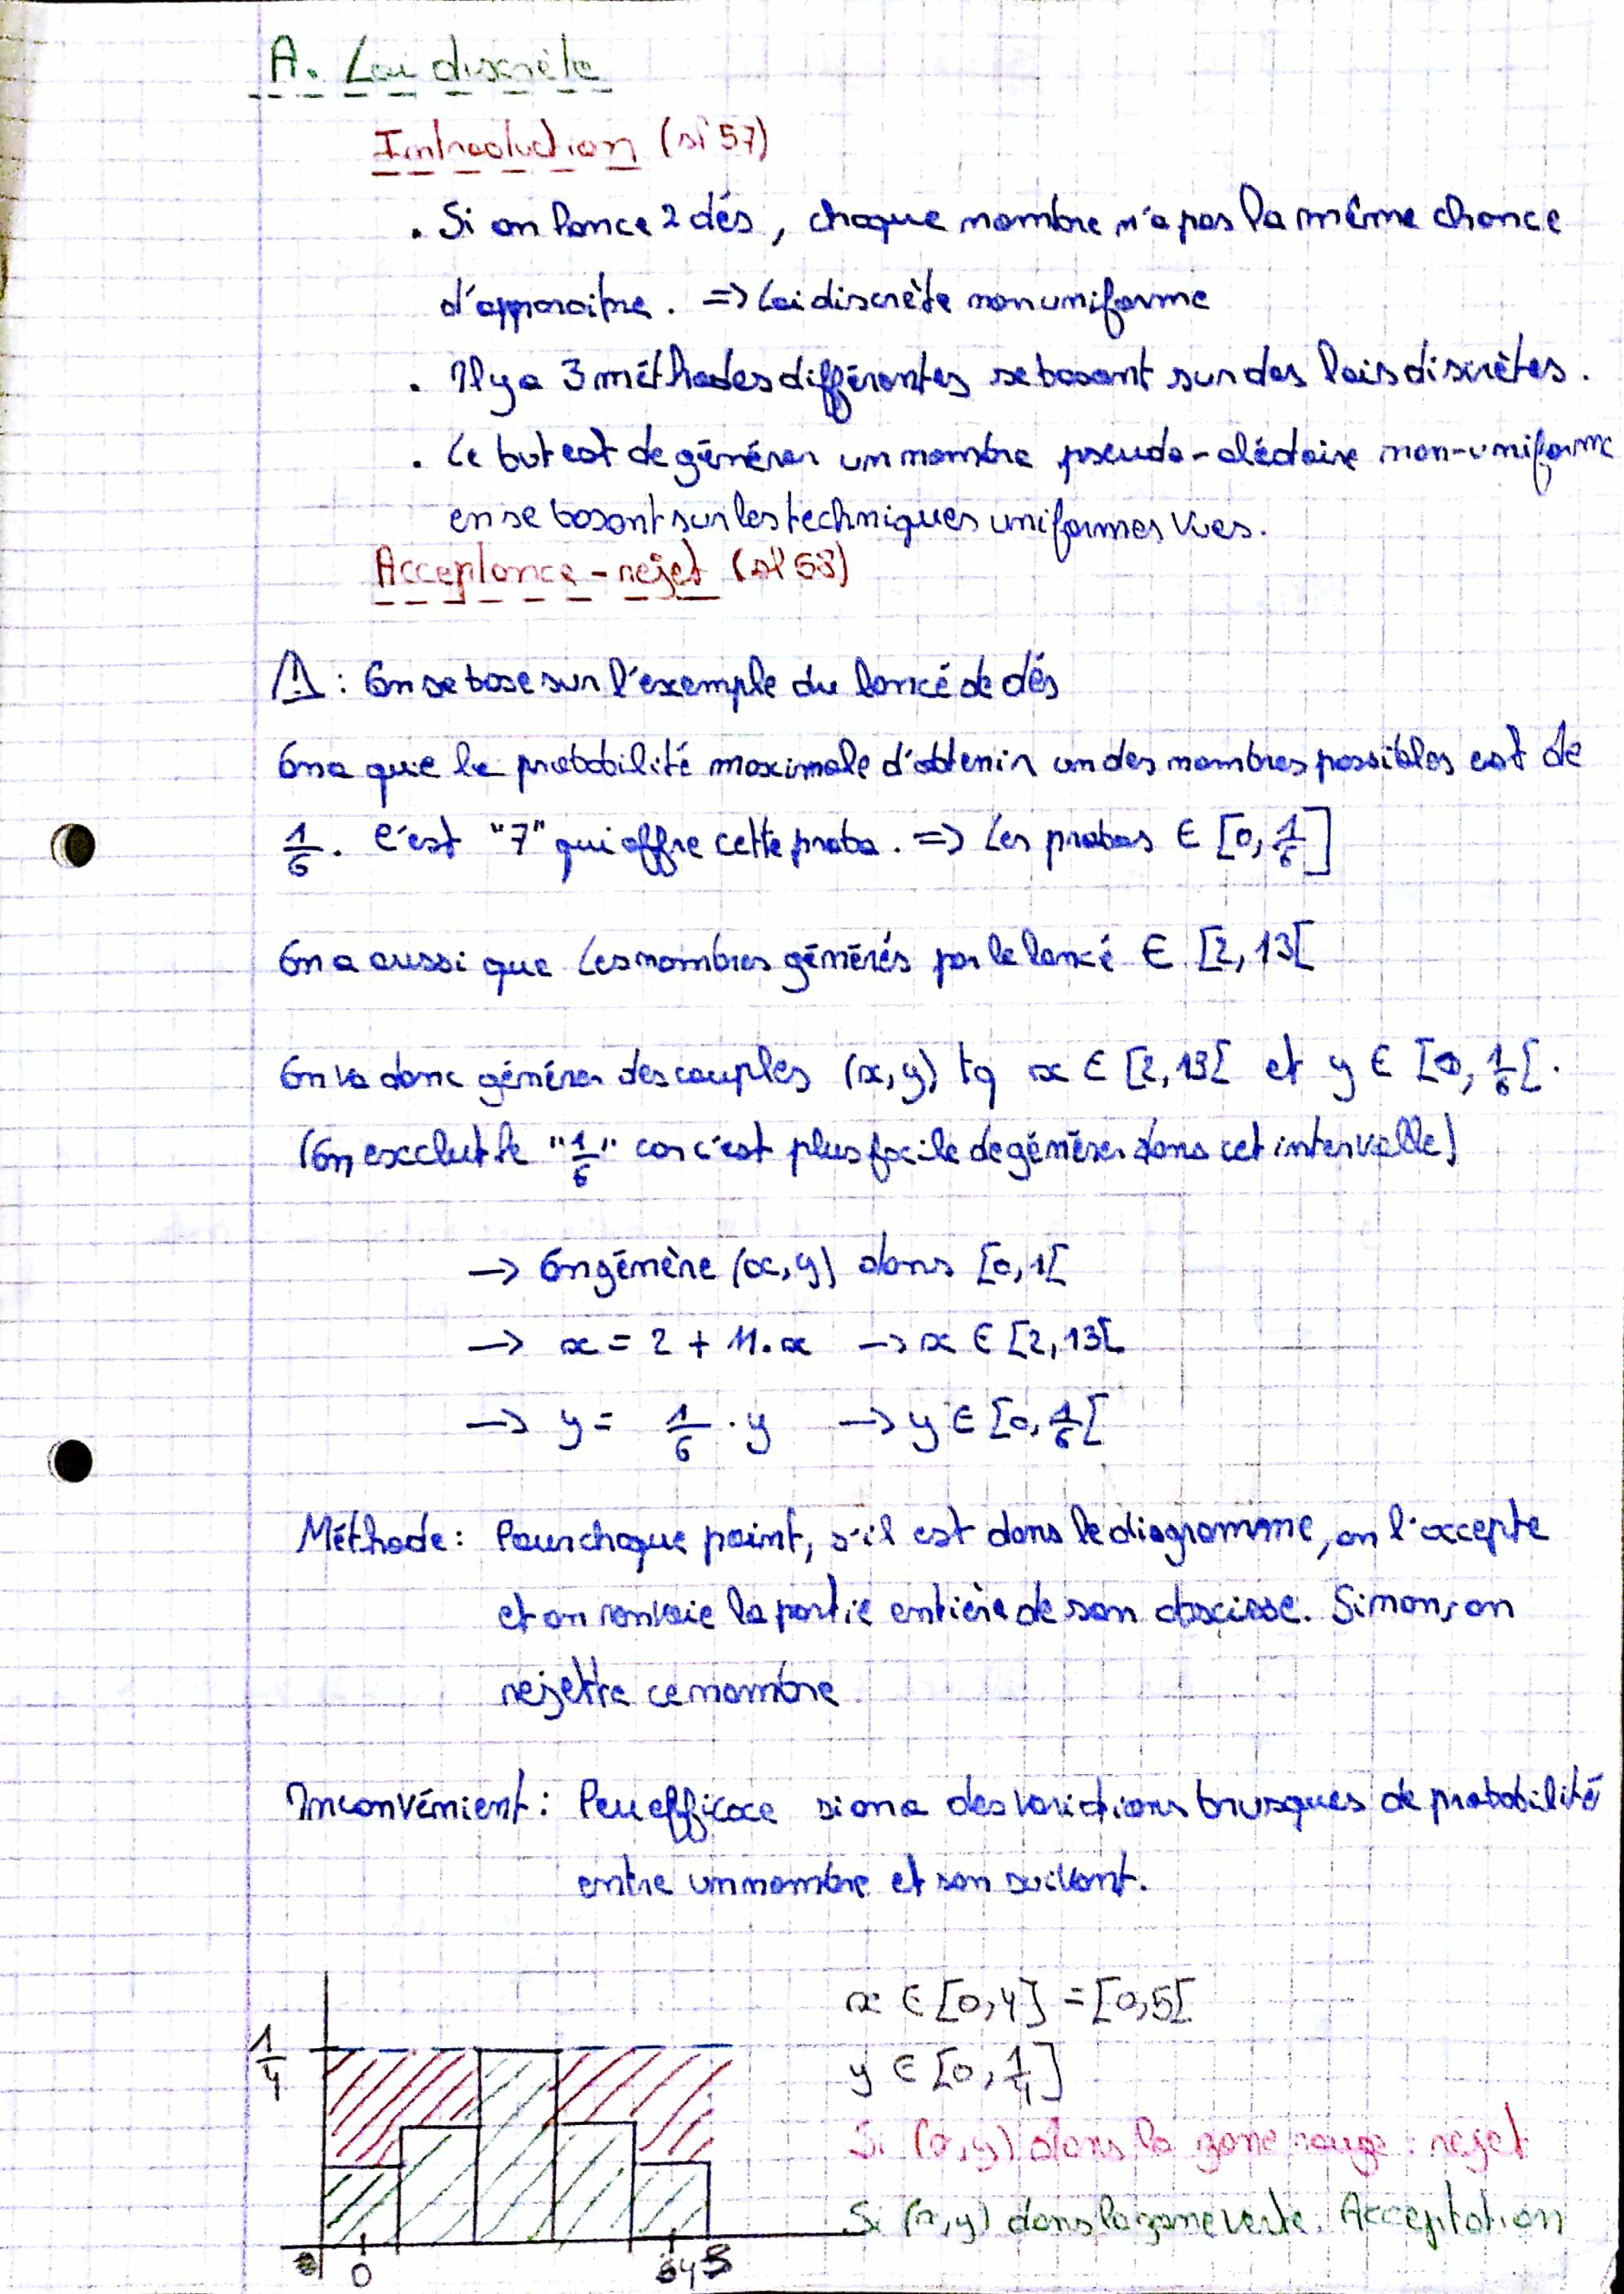
\includegraphics[height=\textheight-1.16cm]{Jonathan(1)}
\end{figure}
\begin{figure}[H]
    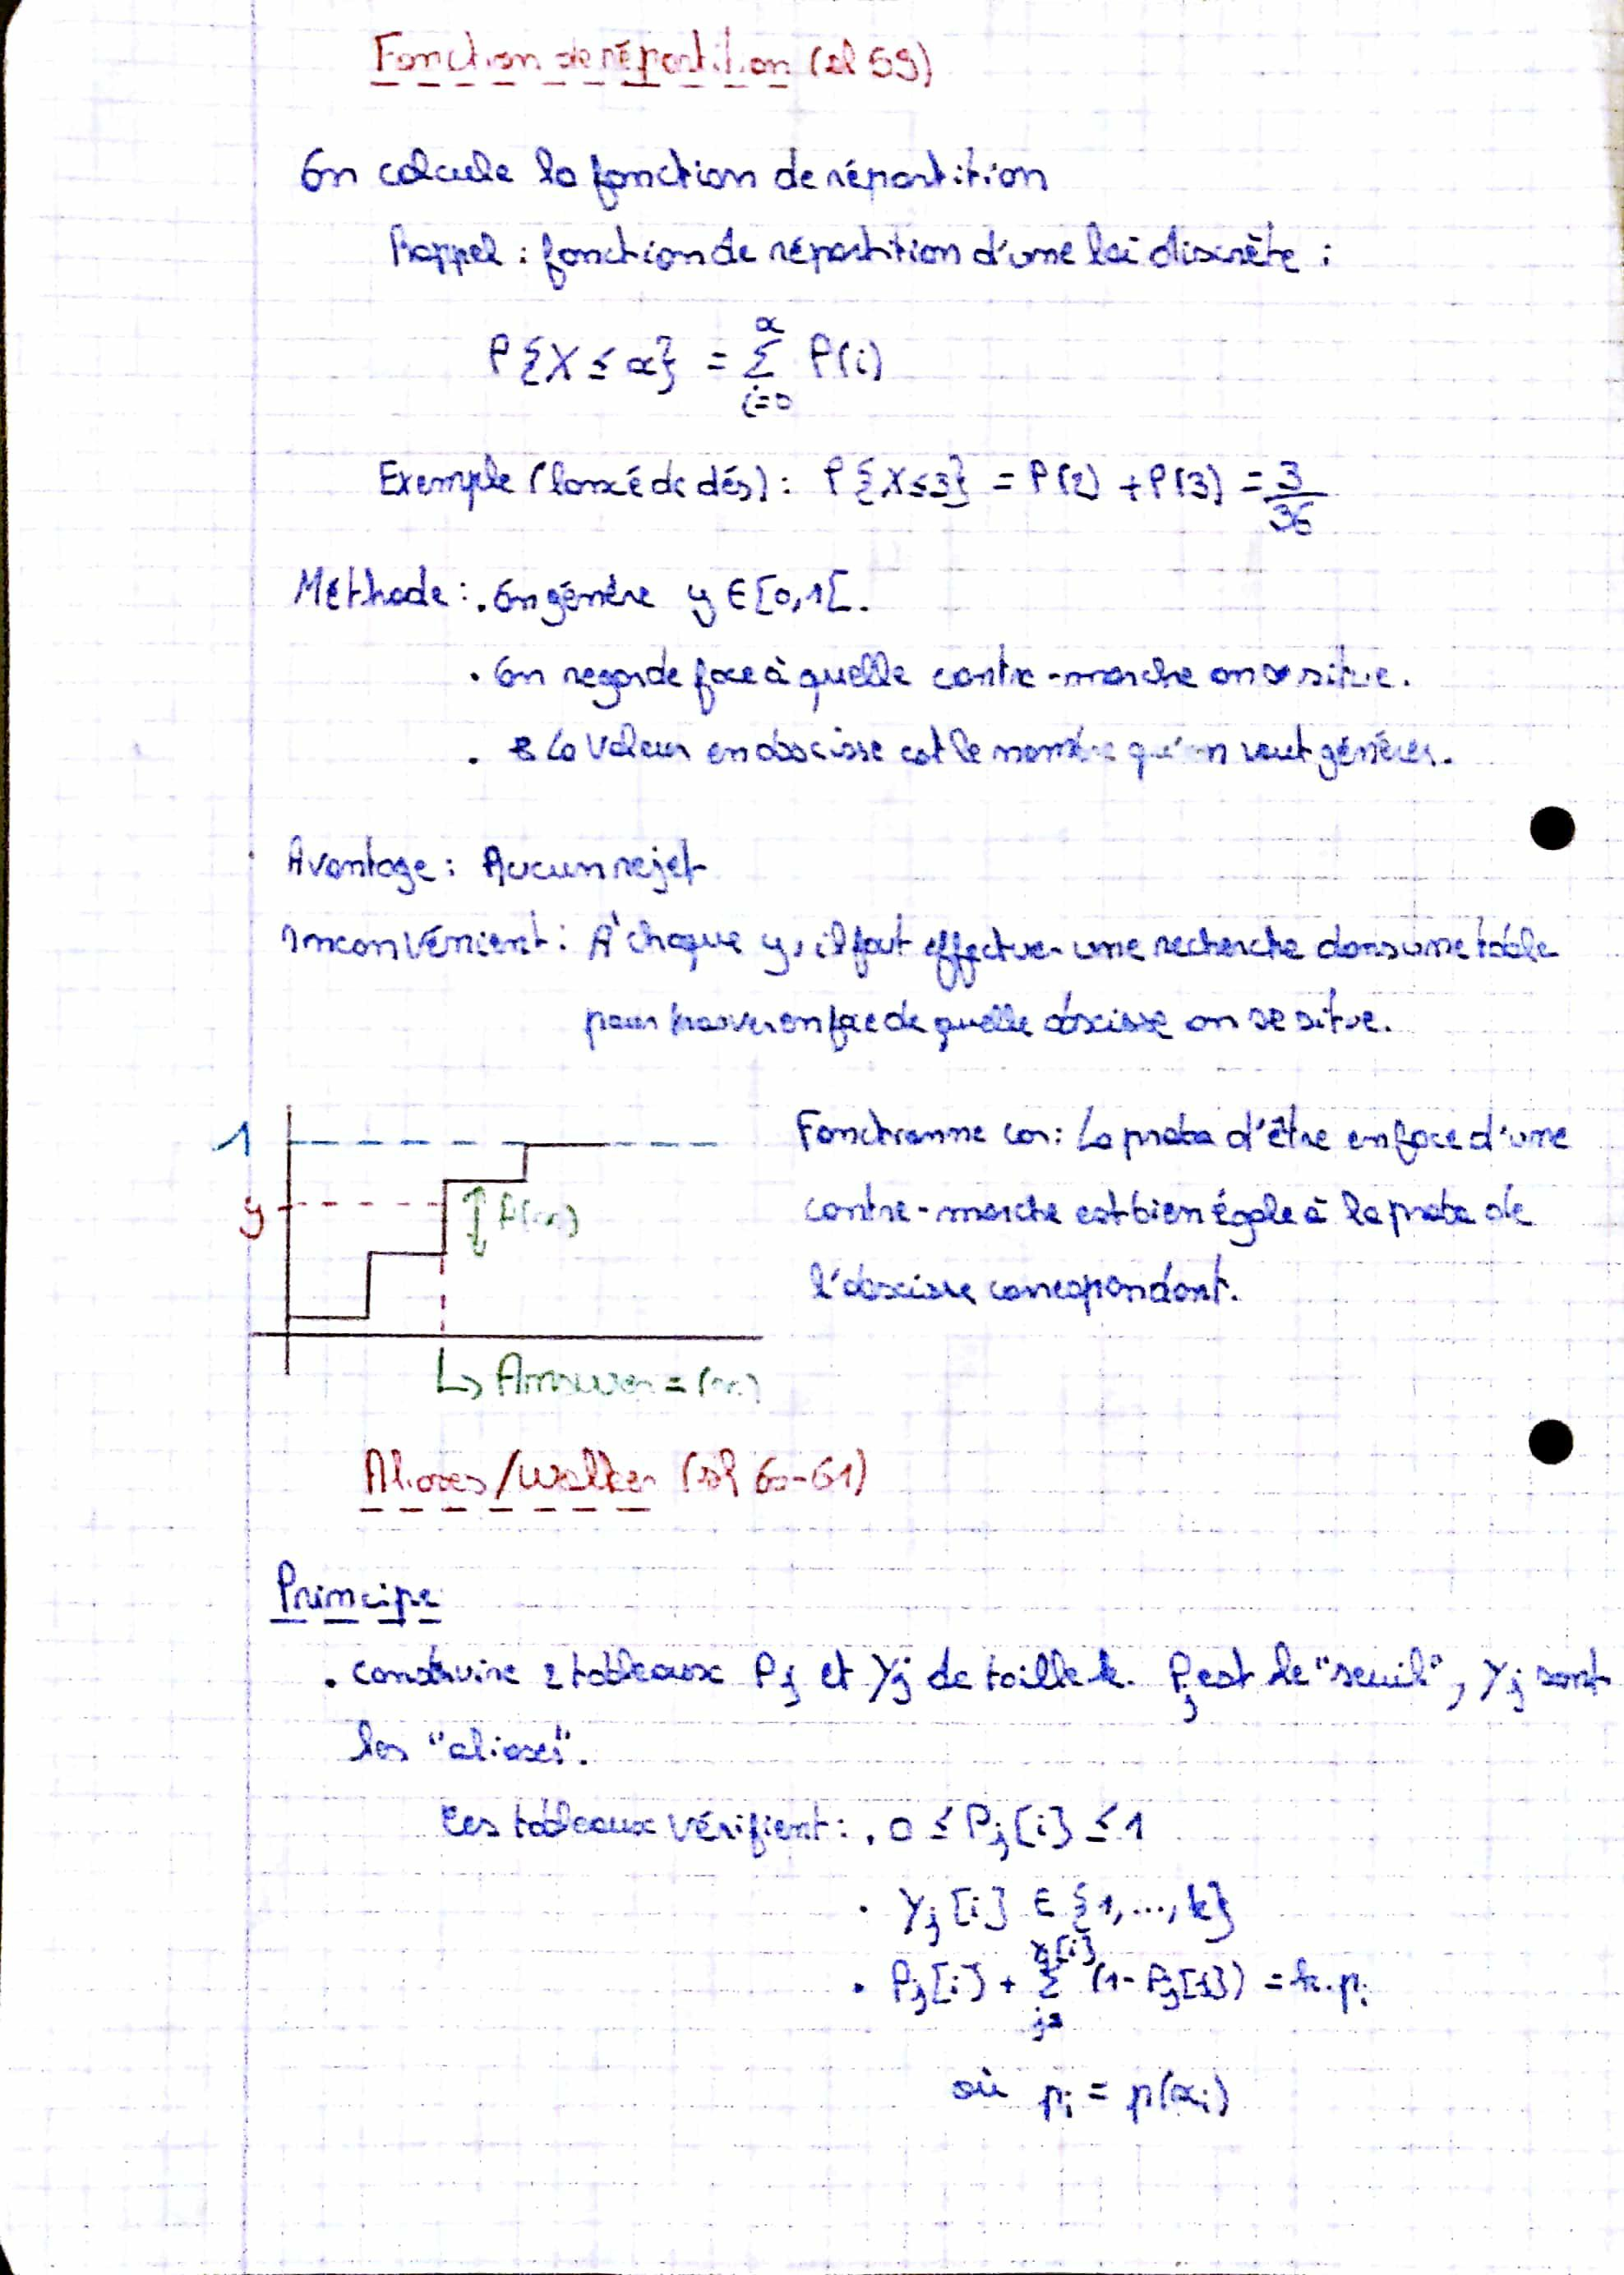
\includegraphics[width=\textwidth]{Jonathan(2)}
\end{figure}
\begin{figure}[H]
    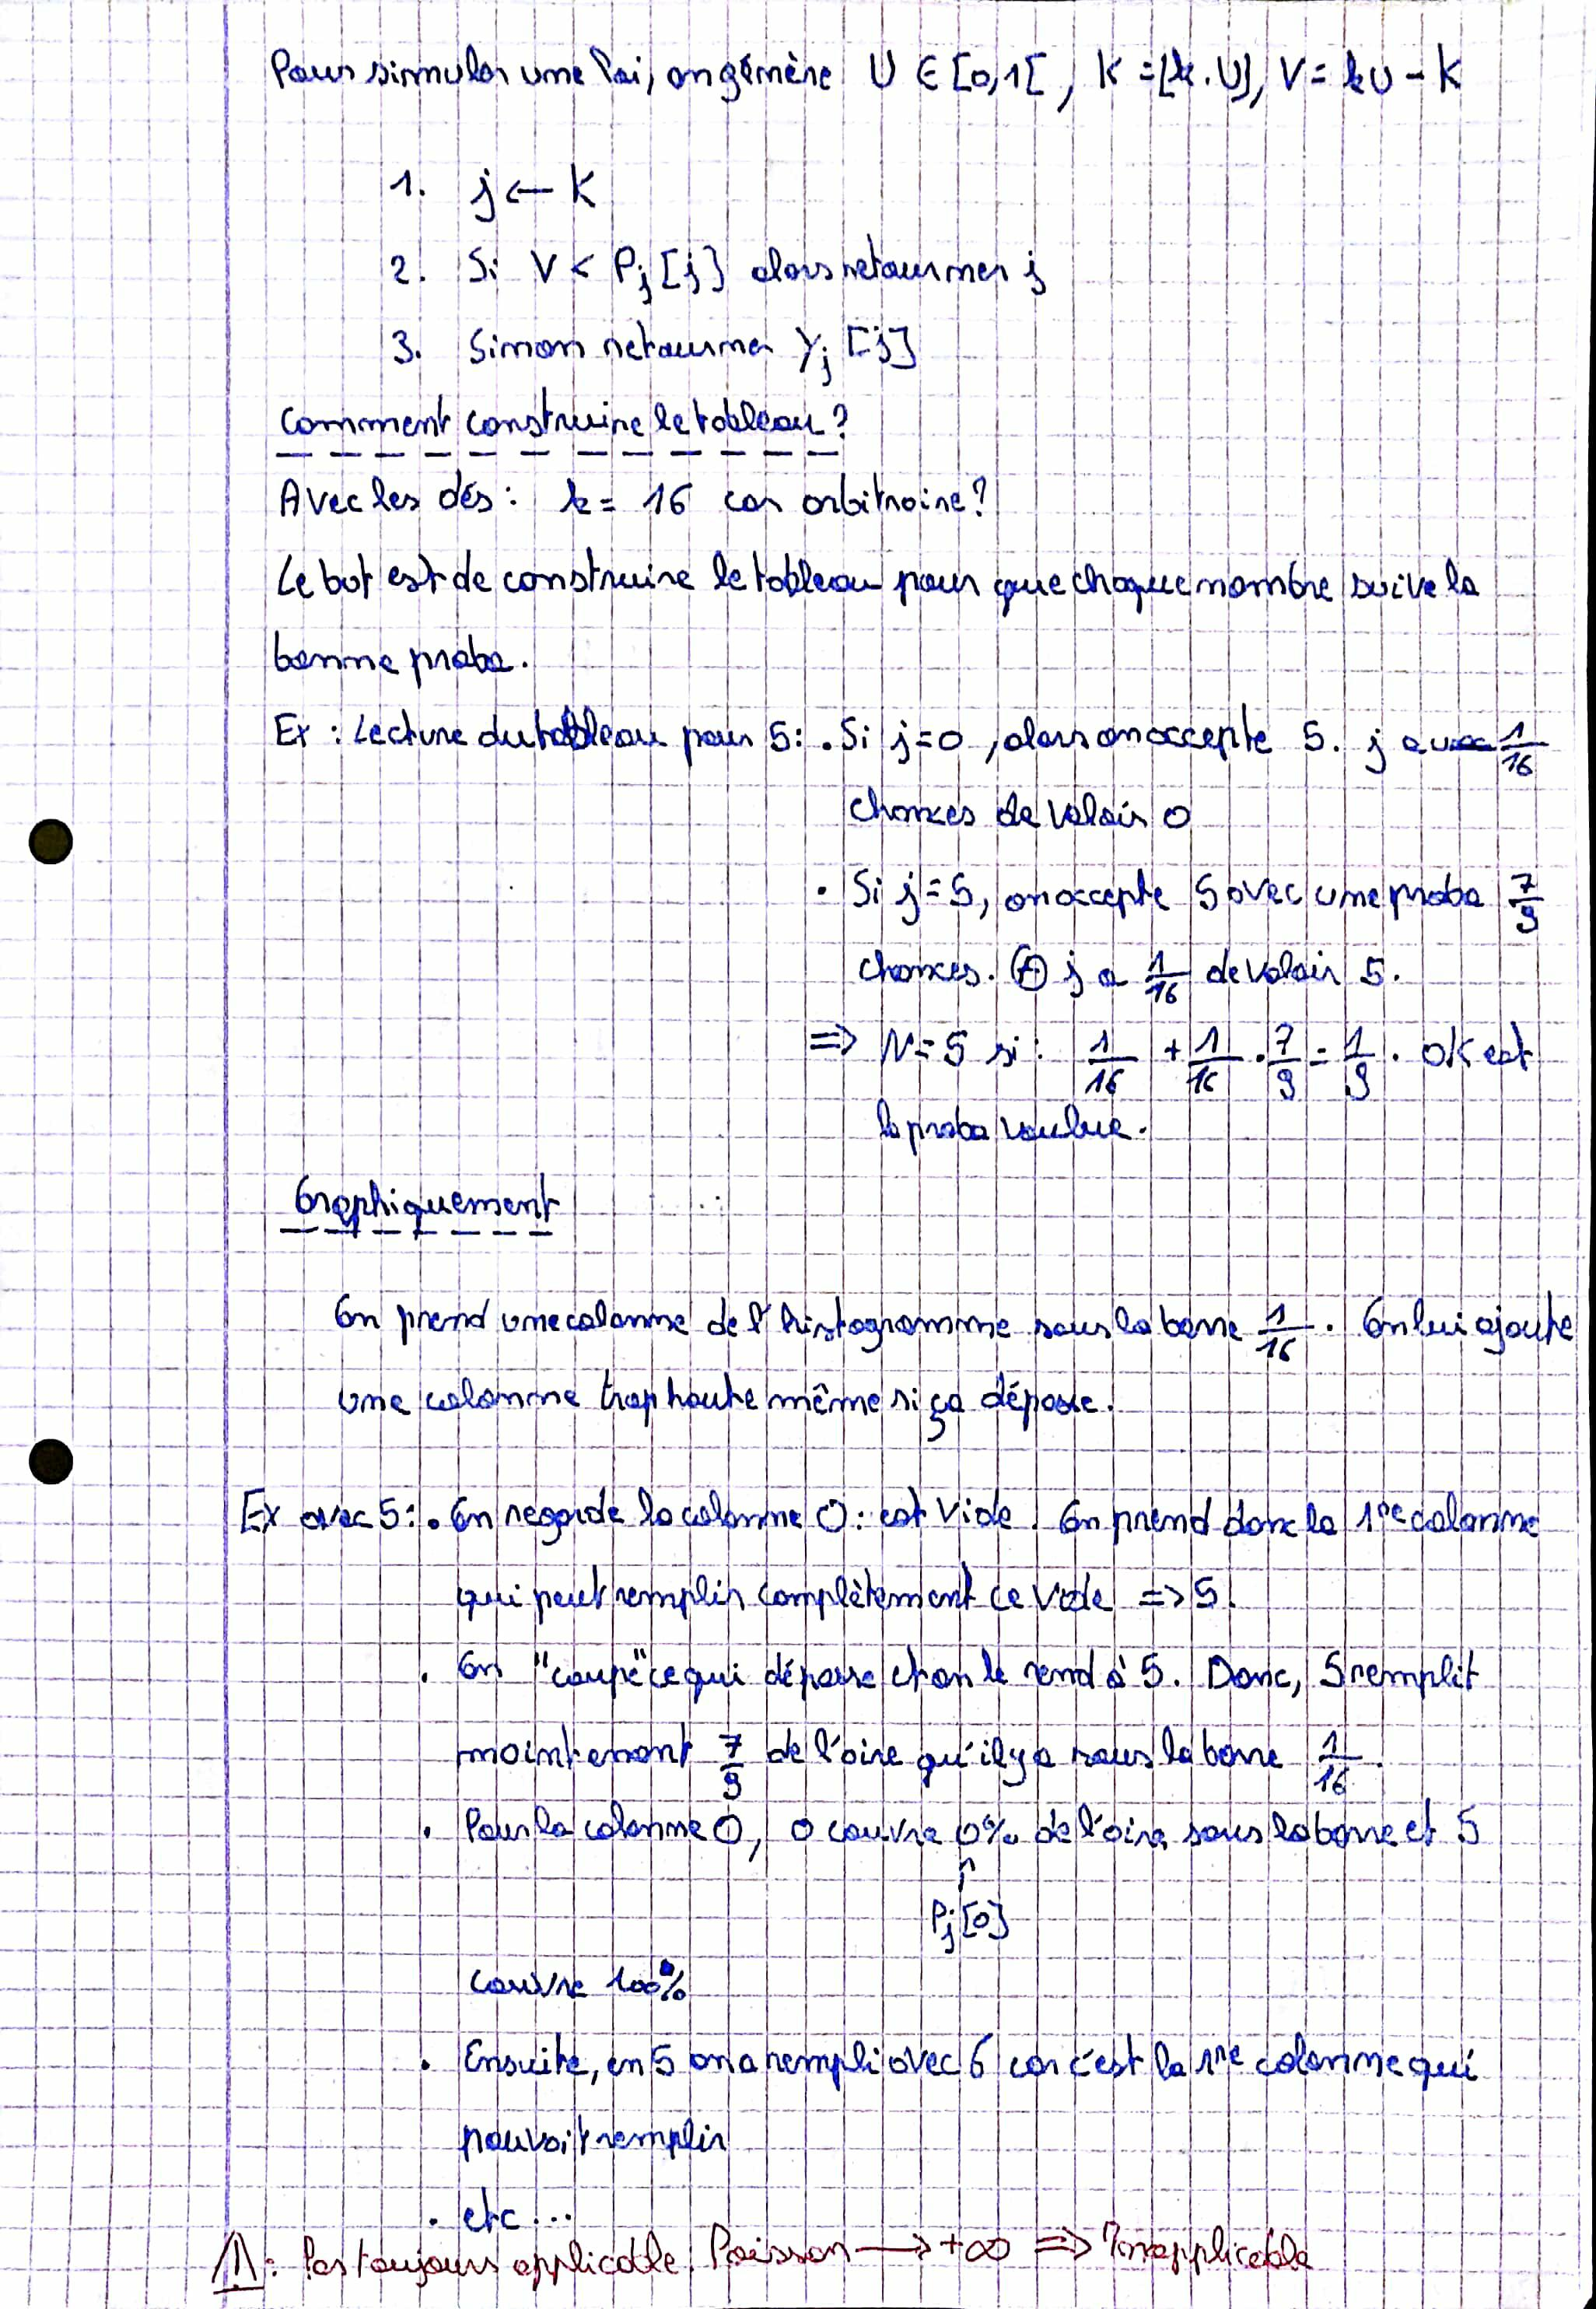
\includegraphics[width=\textwidth]{Jonathan(3)}
\end{figure}
\section{Lois continues}
\subsection{Acceptance-rejet et inversion de la fonction de répartition}
\begin{figure}[H]
    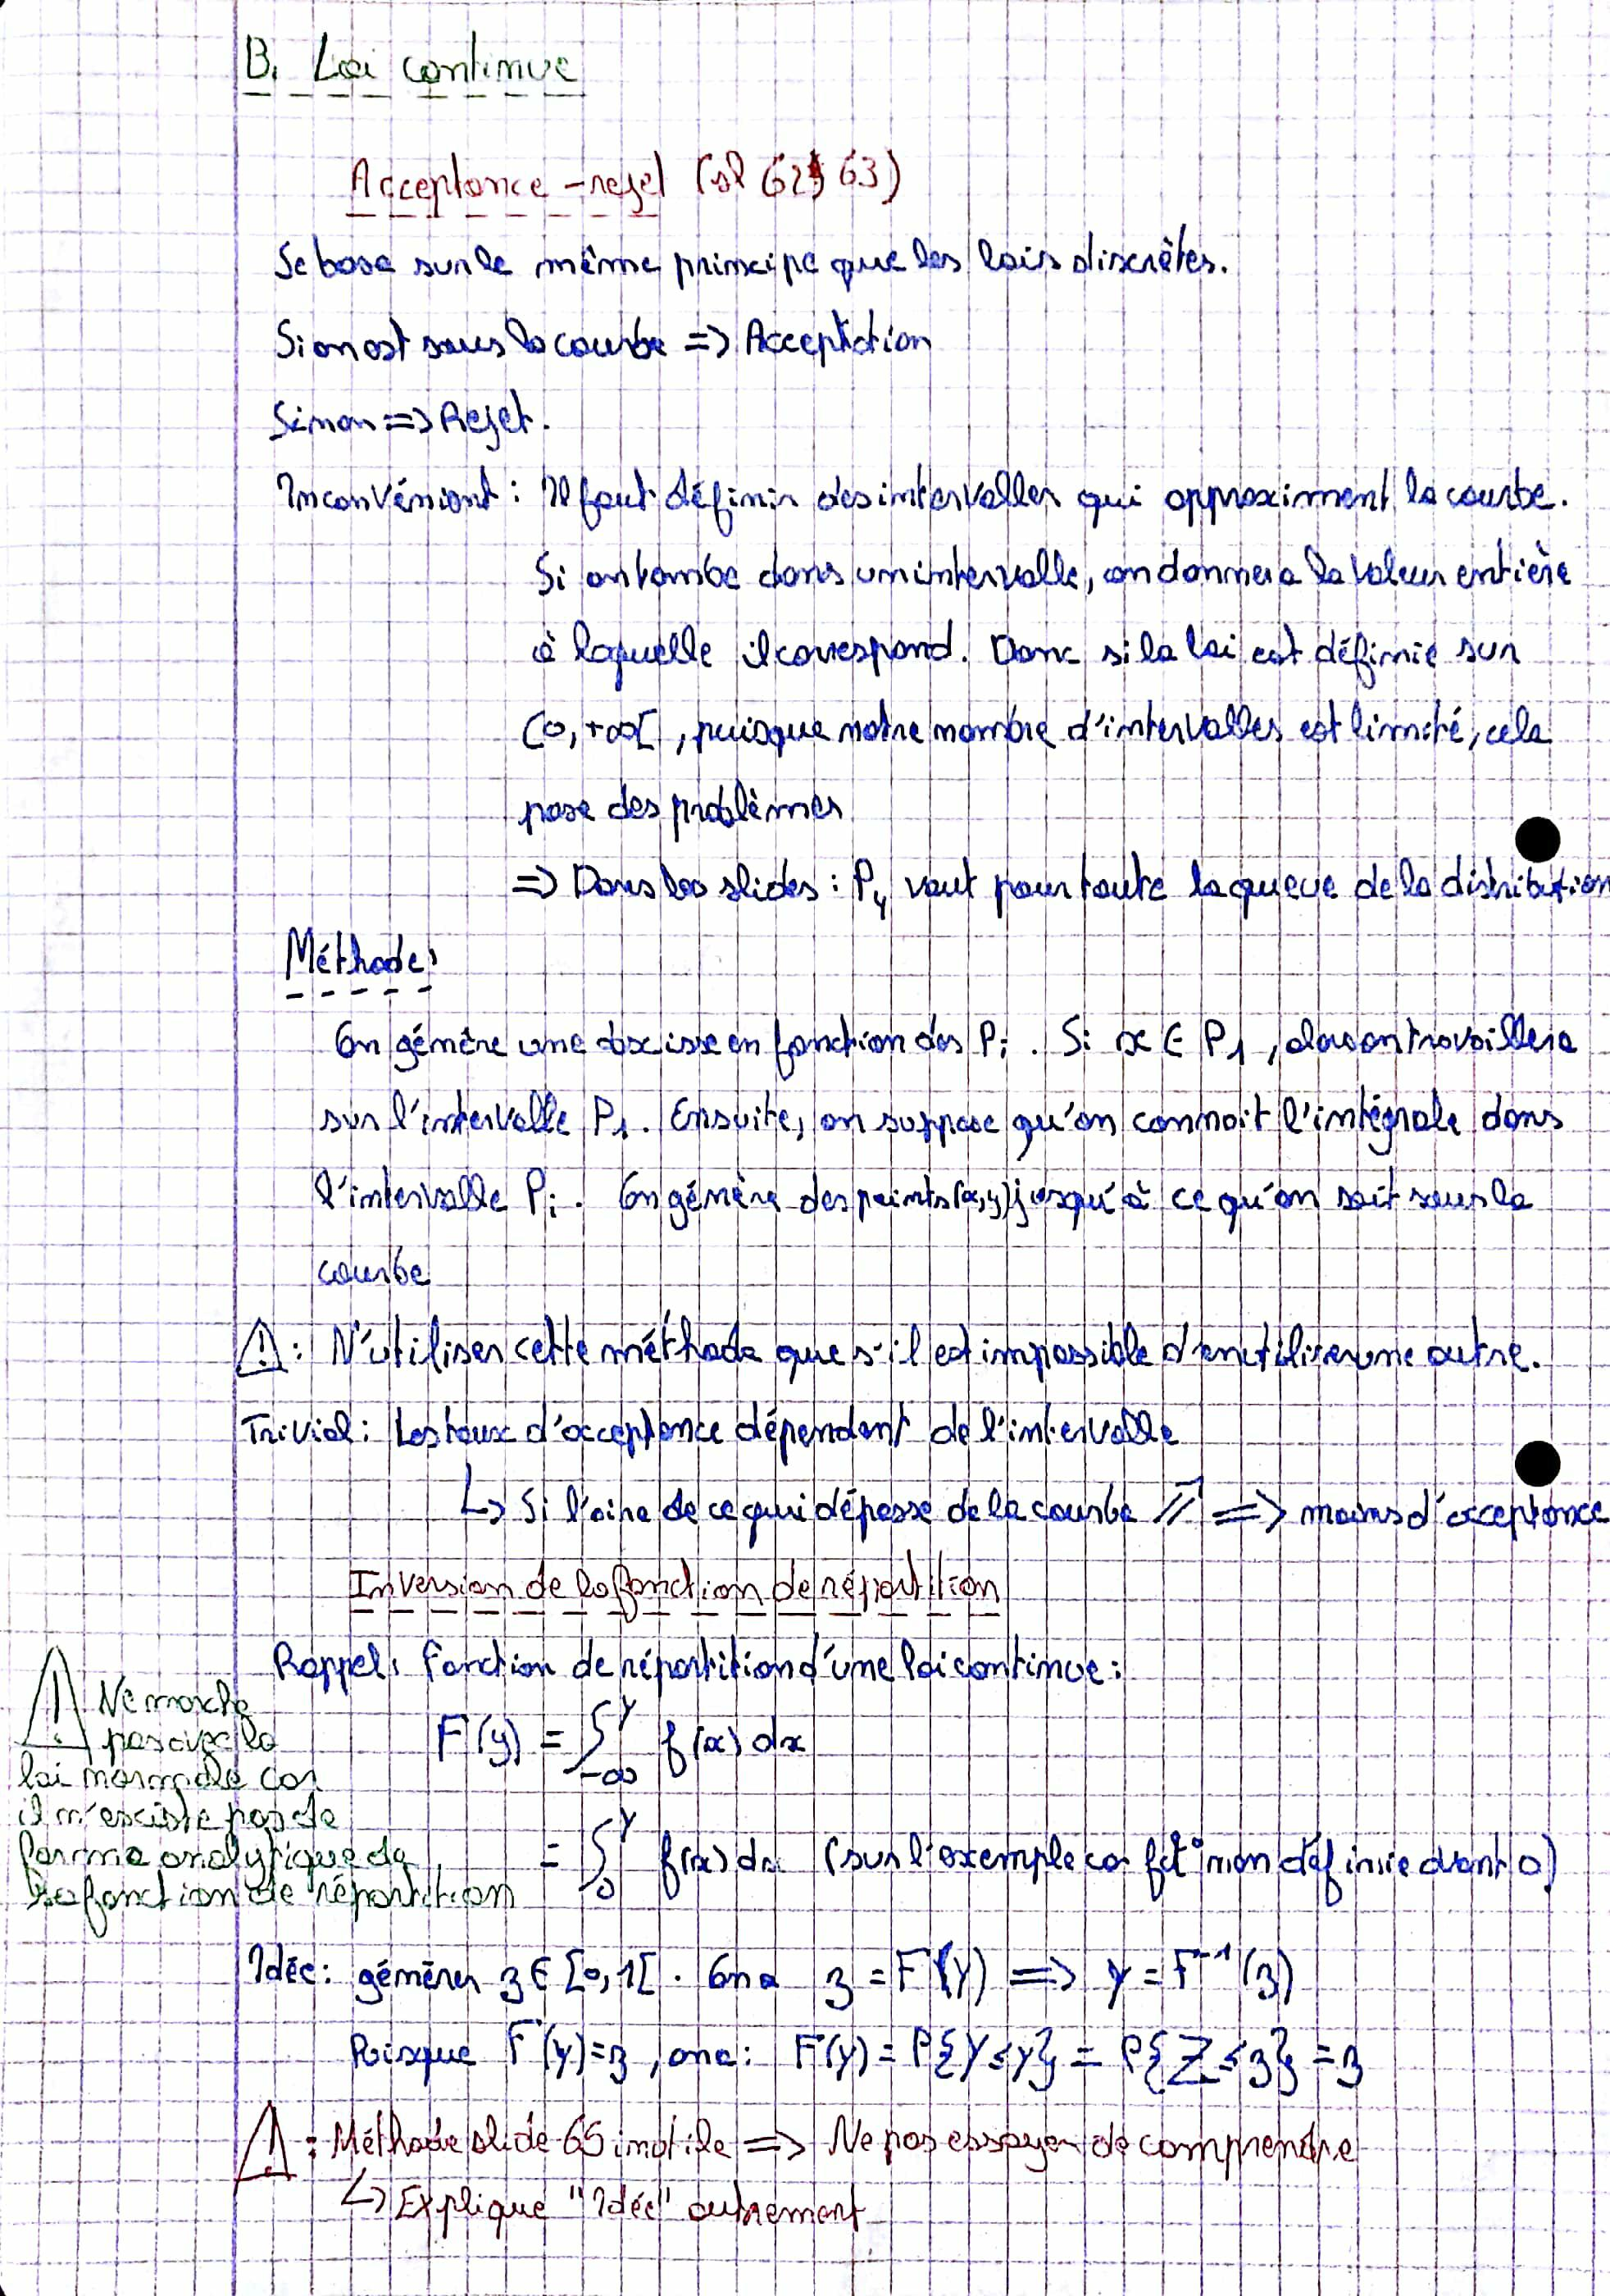
\includegraphics[width=\textwidth-1.16cm]{Jonathan(4)}
\end{figure}
\begin{figure}[H]
    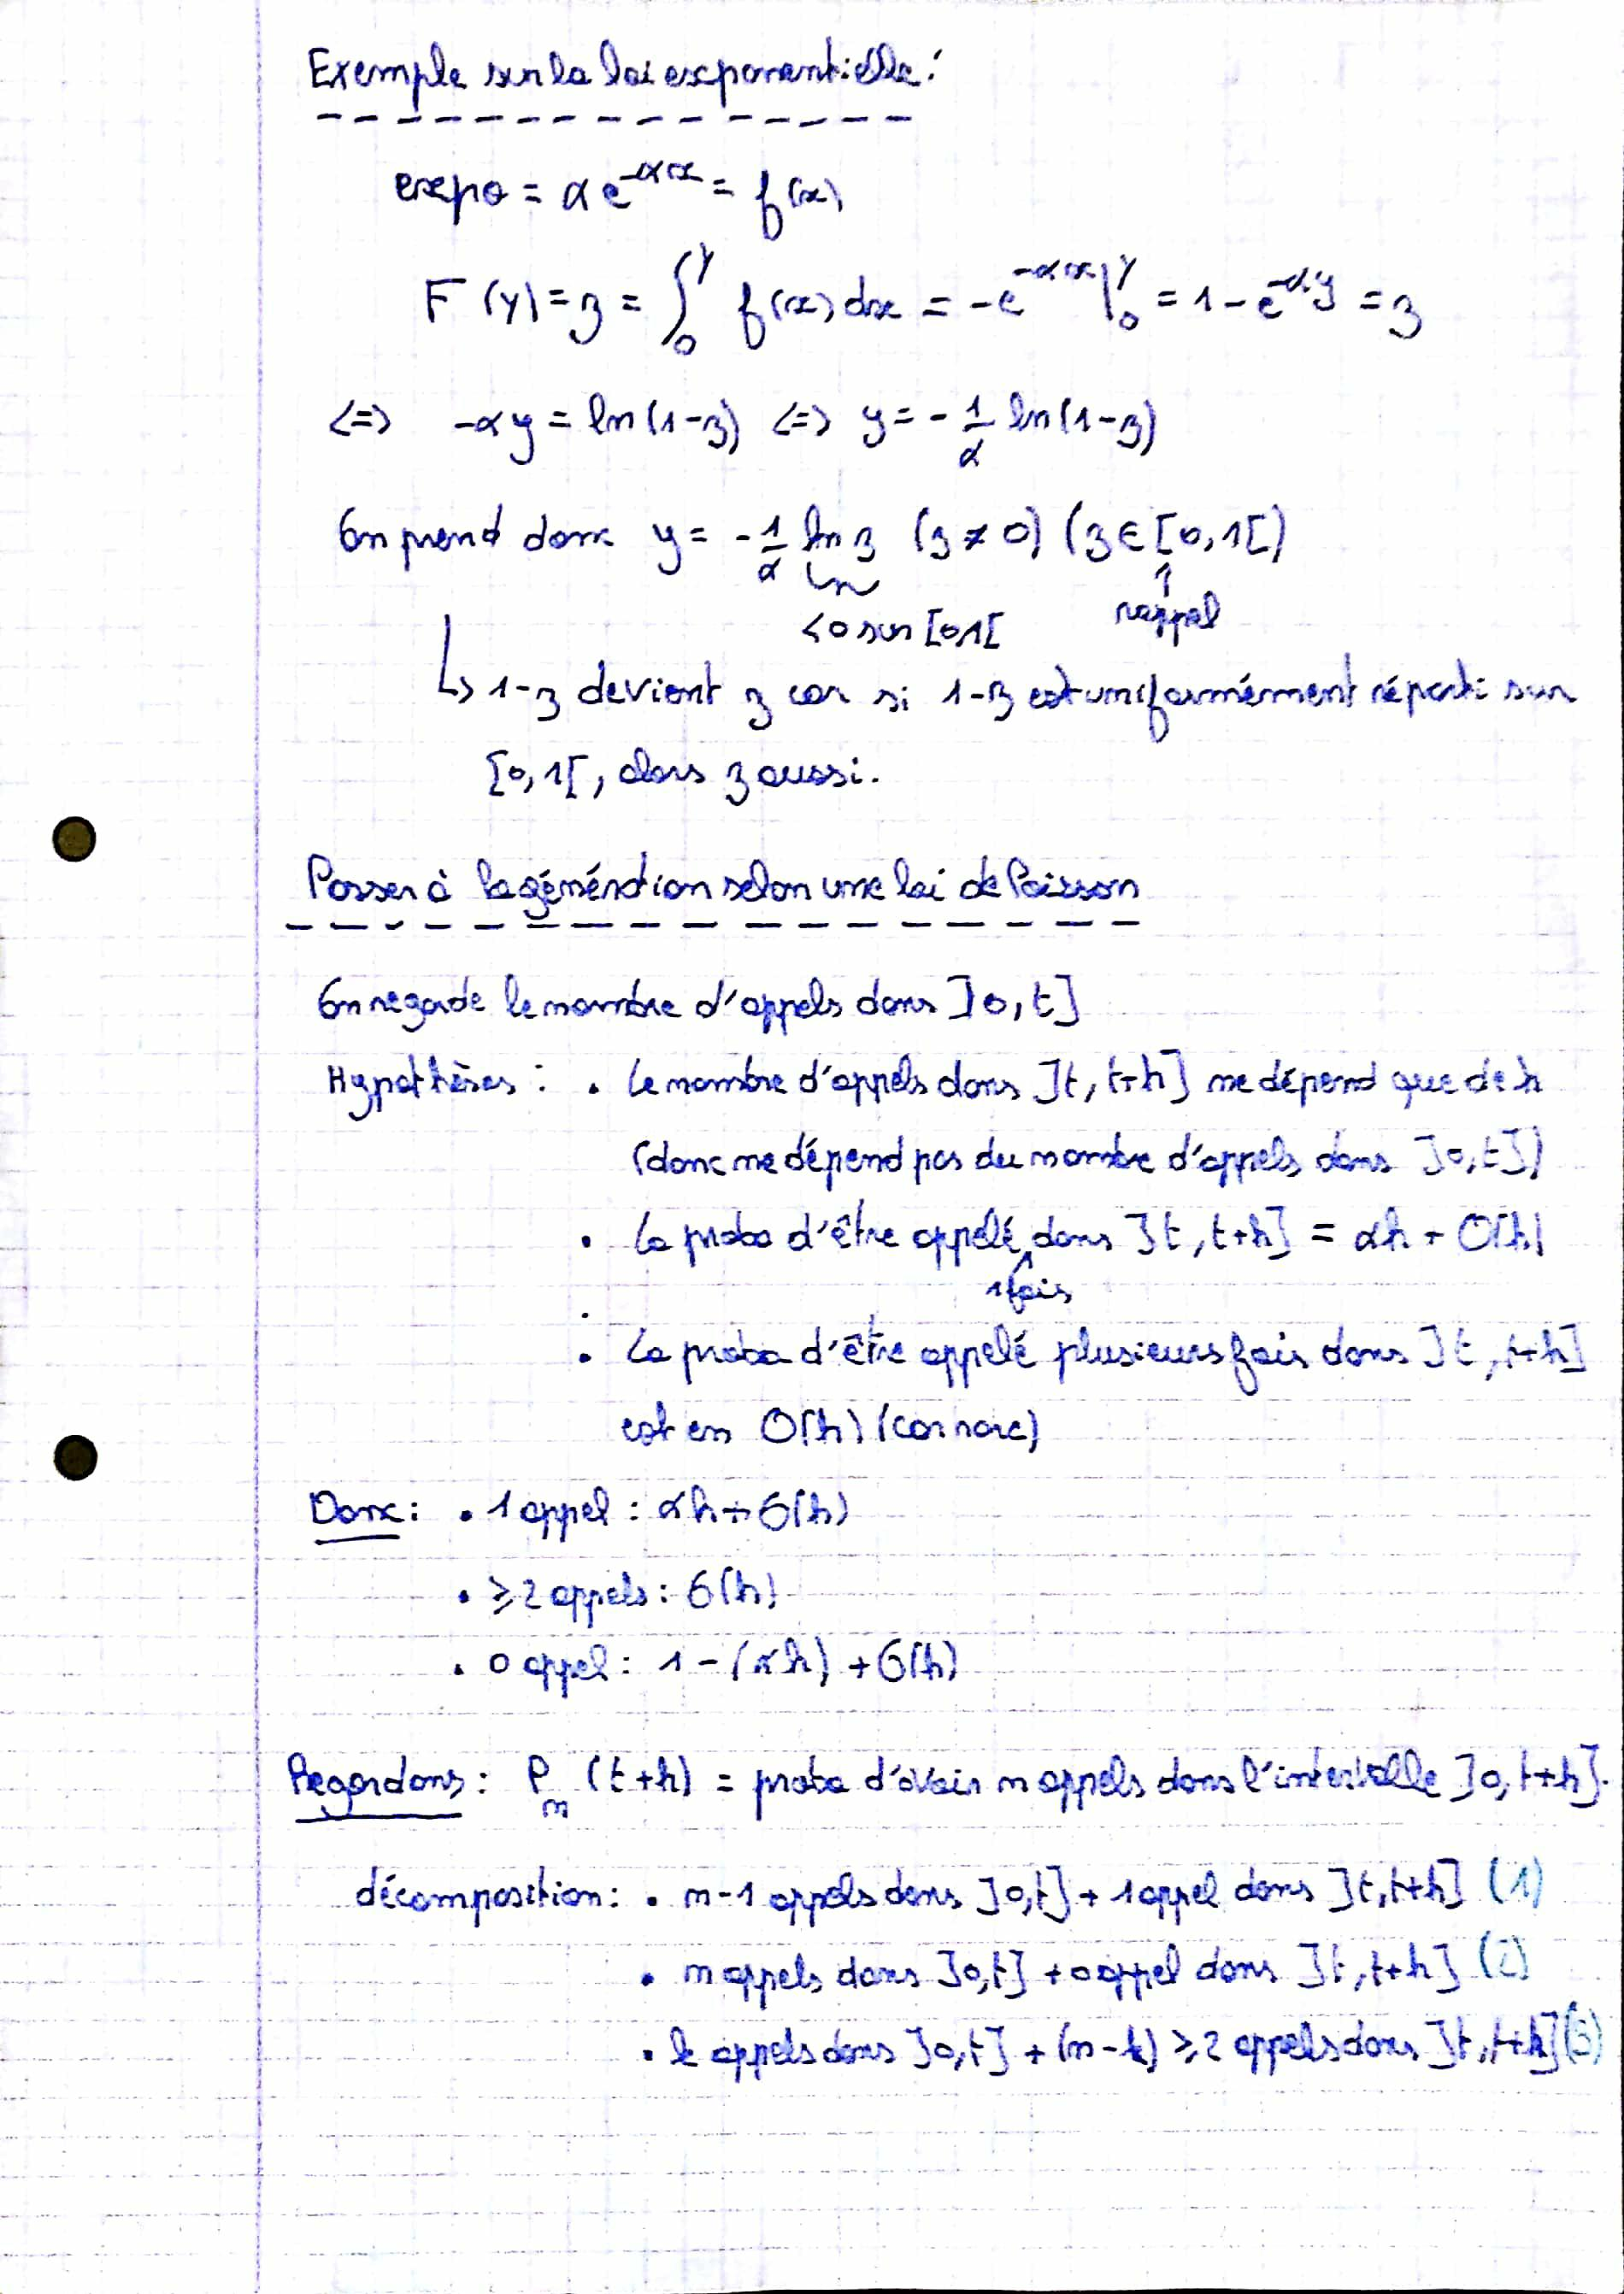
\includegraphics[width=\textwidth]{Jonathan(5)}
\end{figure}
\begin{figure}[H]
    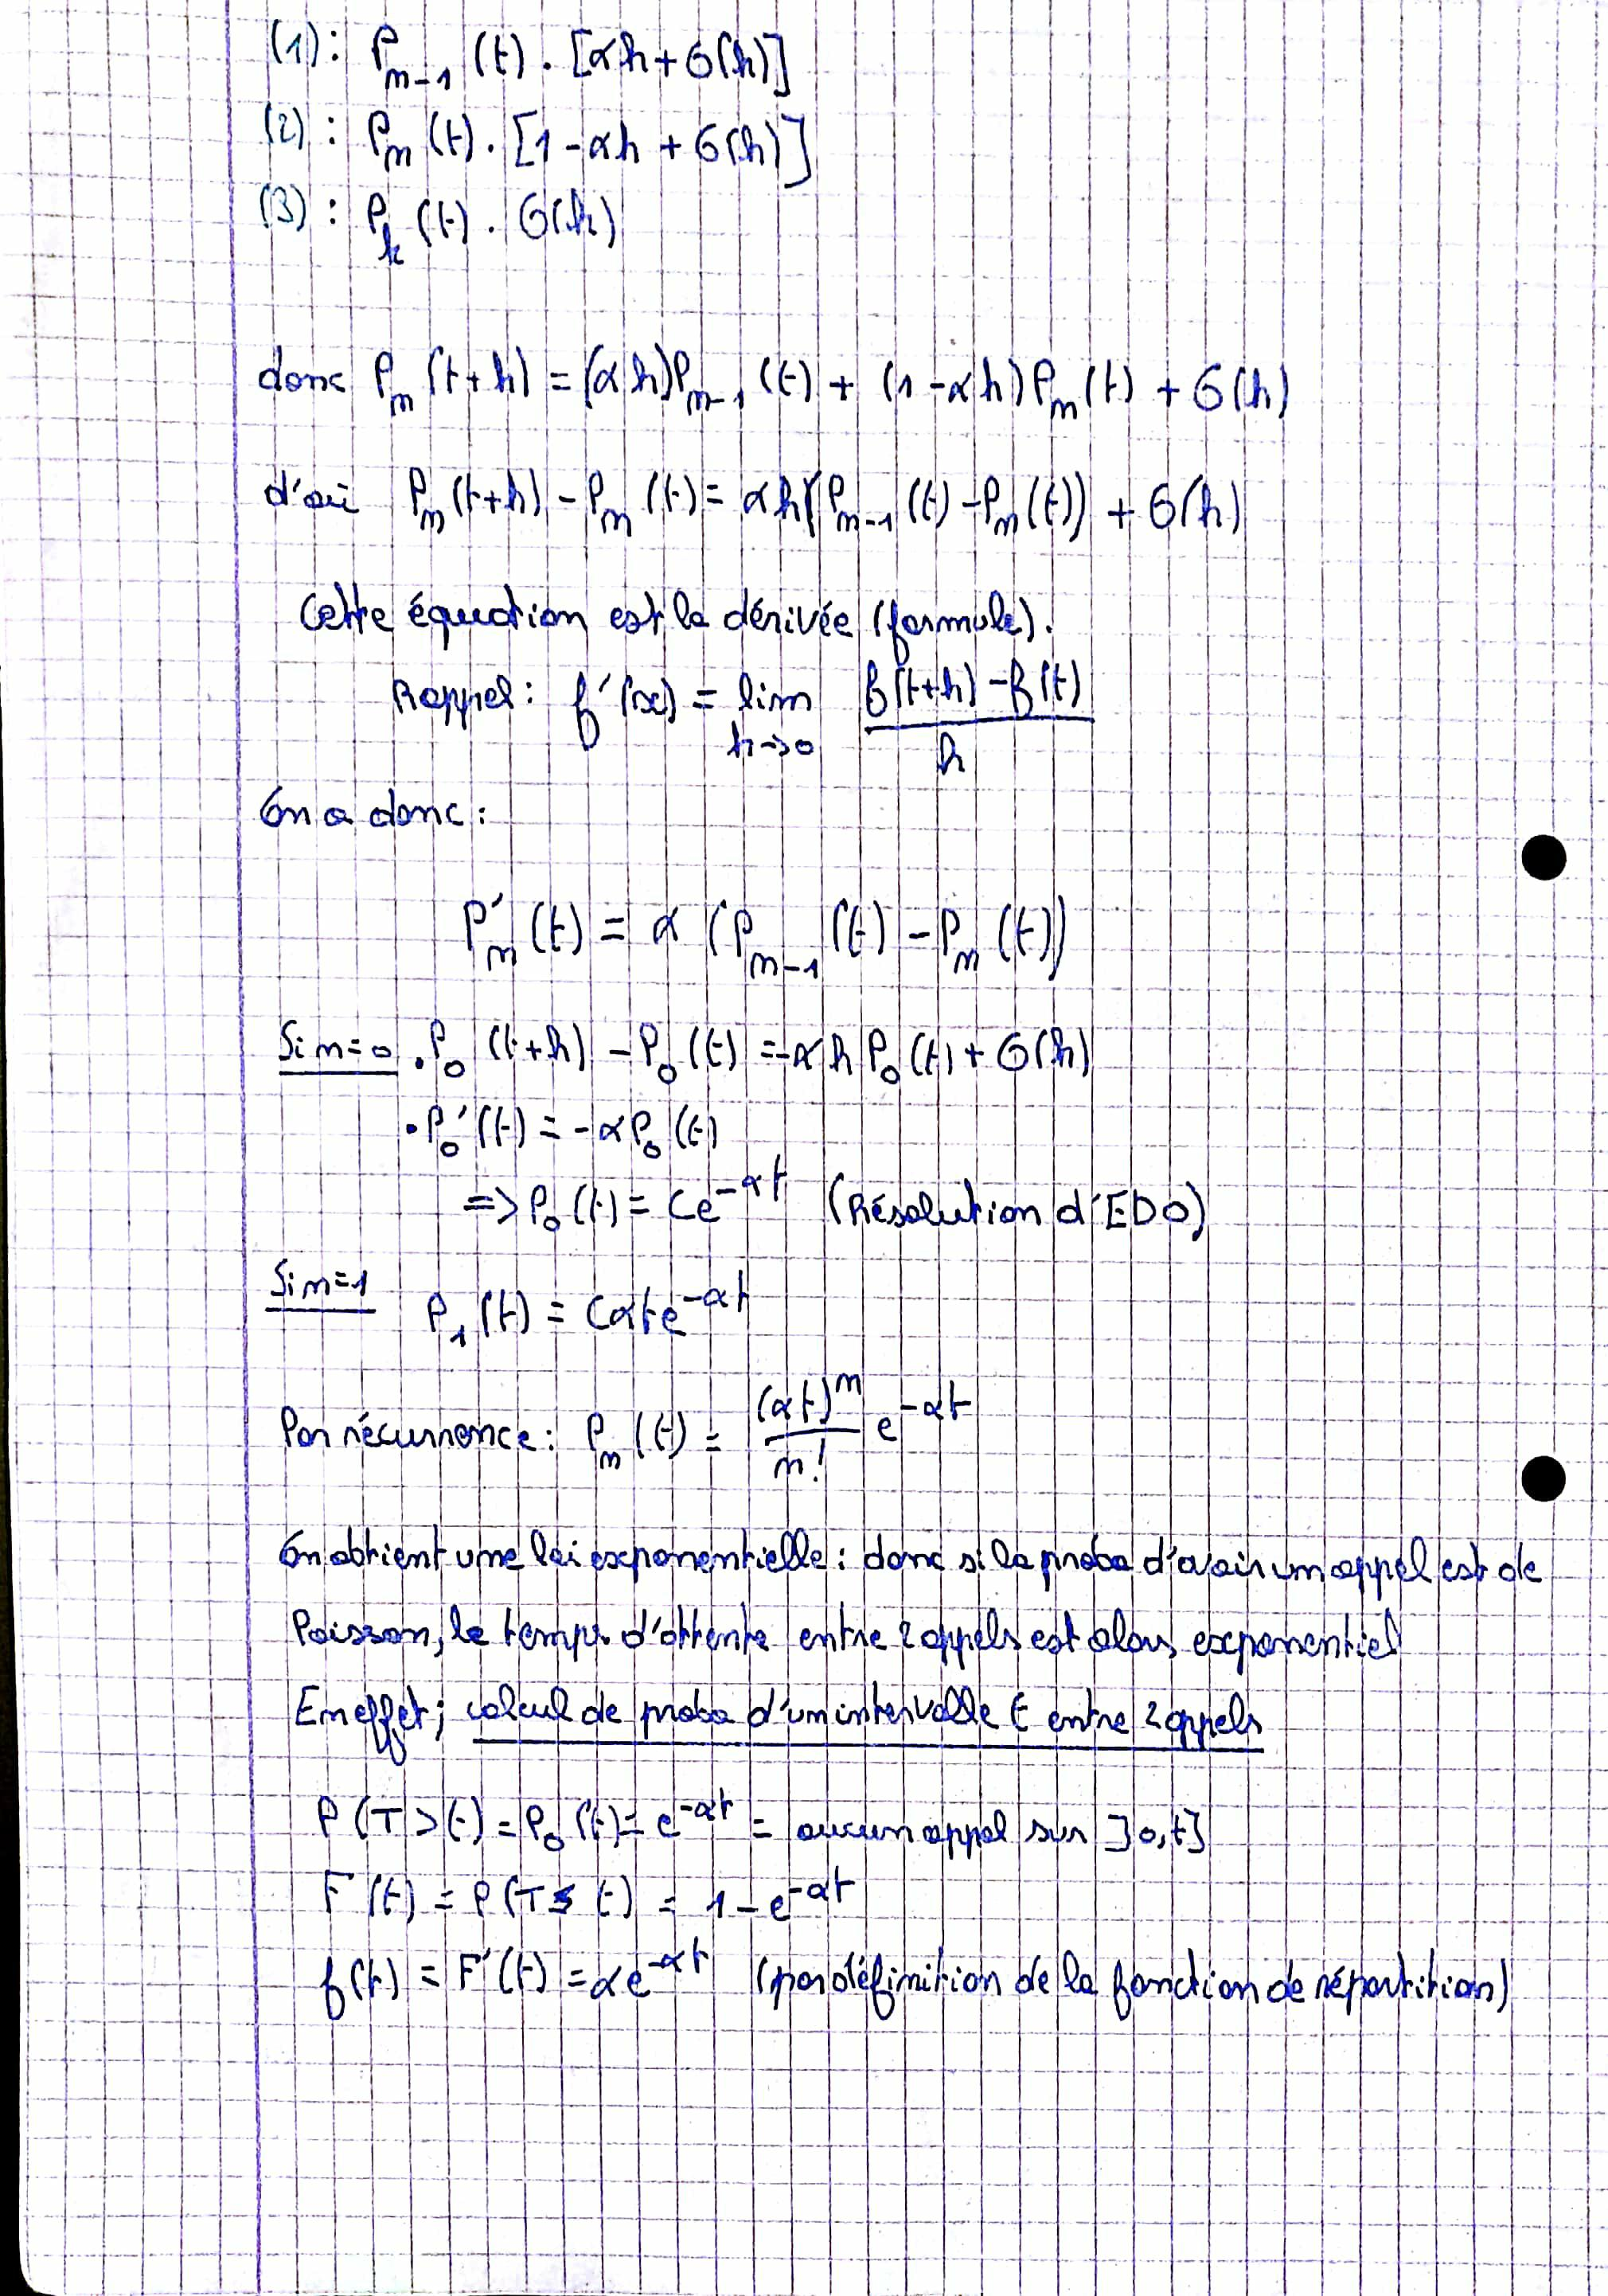
\includegraphics[width=\textwidth]{Jonathan(6)}
\end{figure}
\begin{figure}[H]
    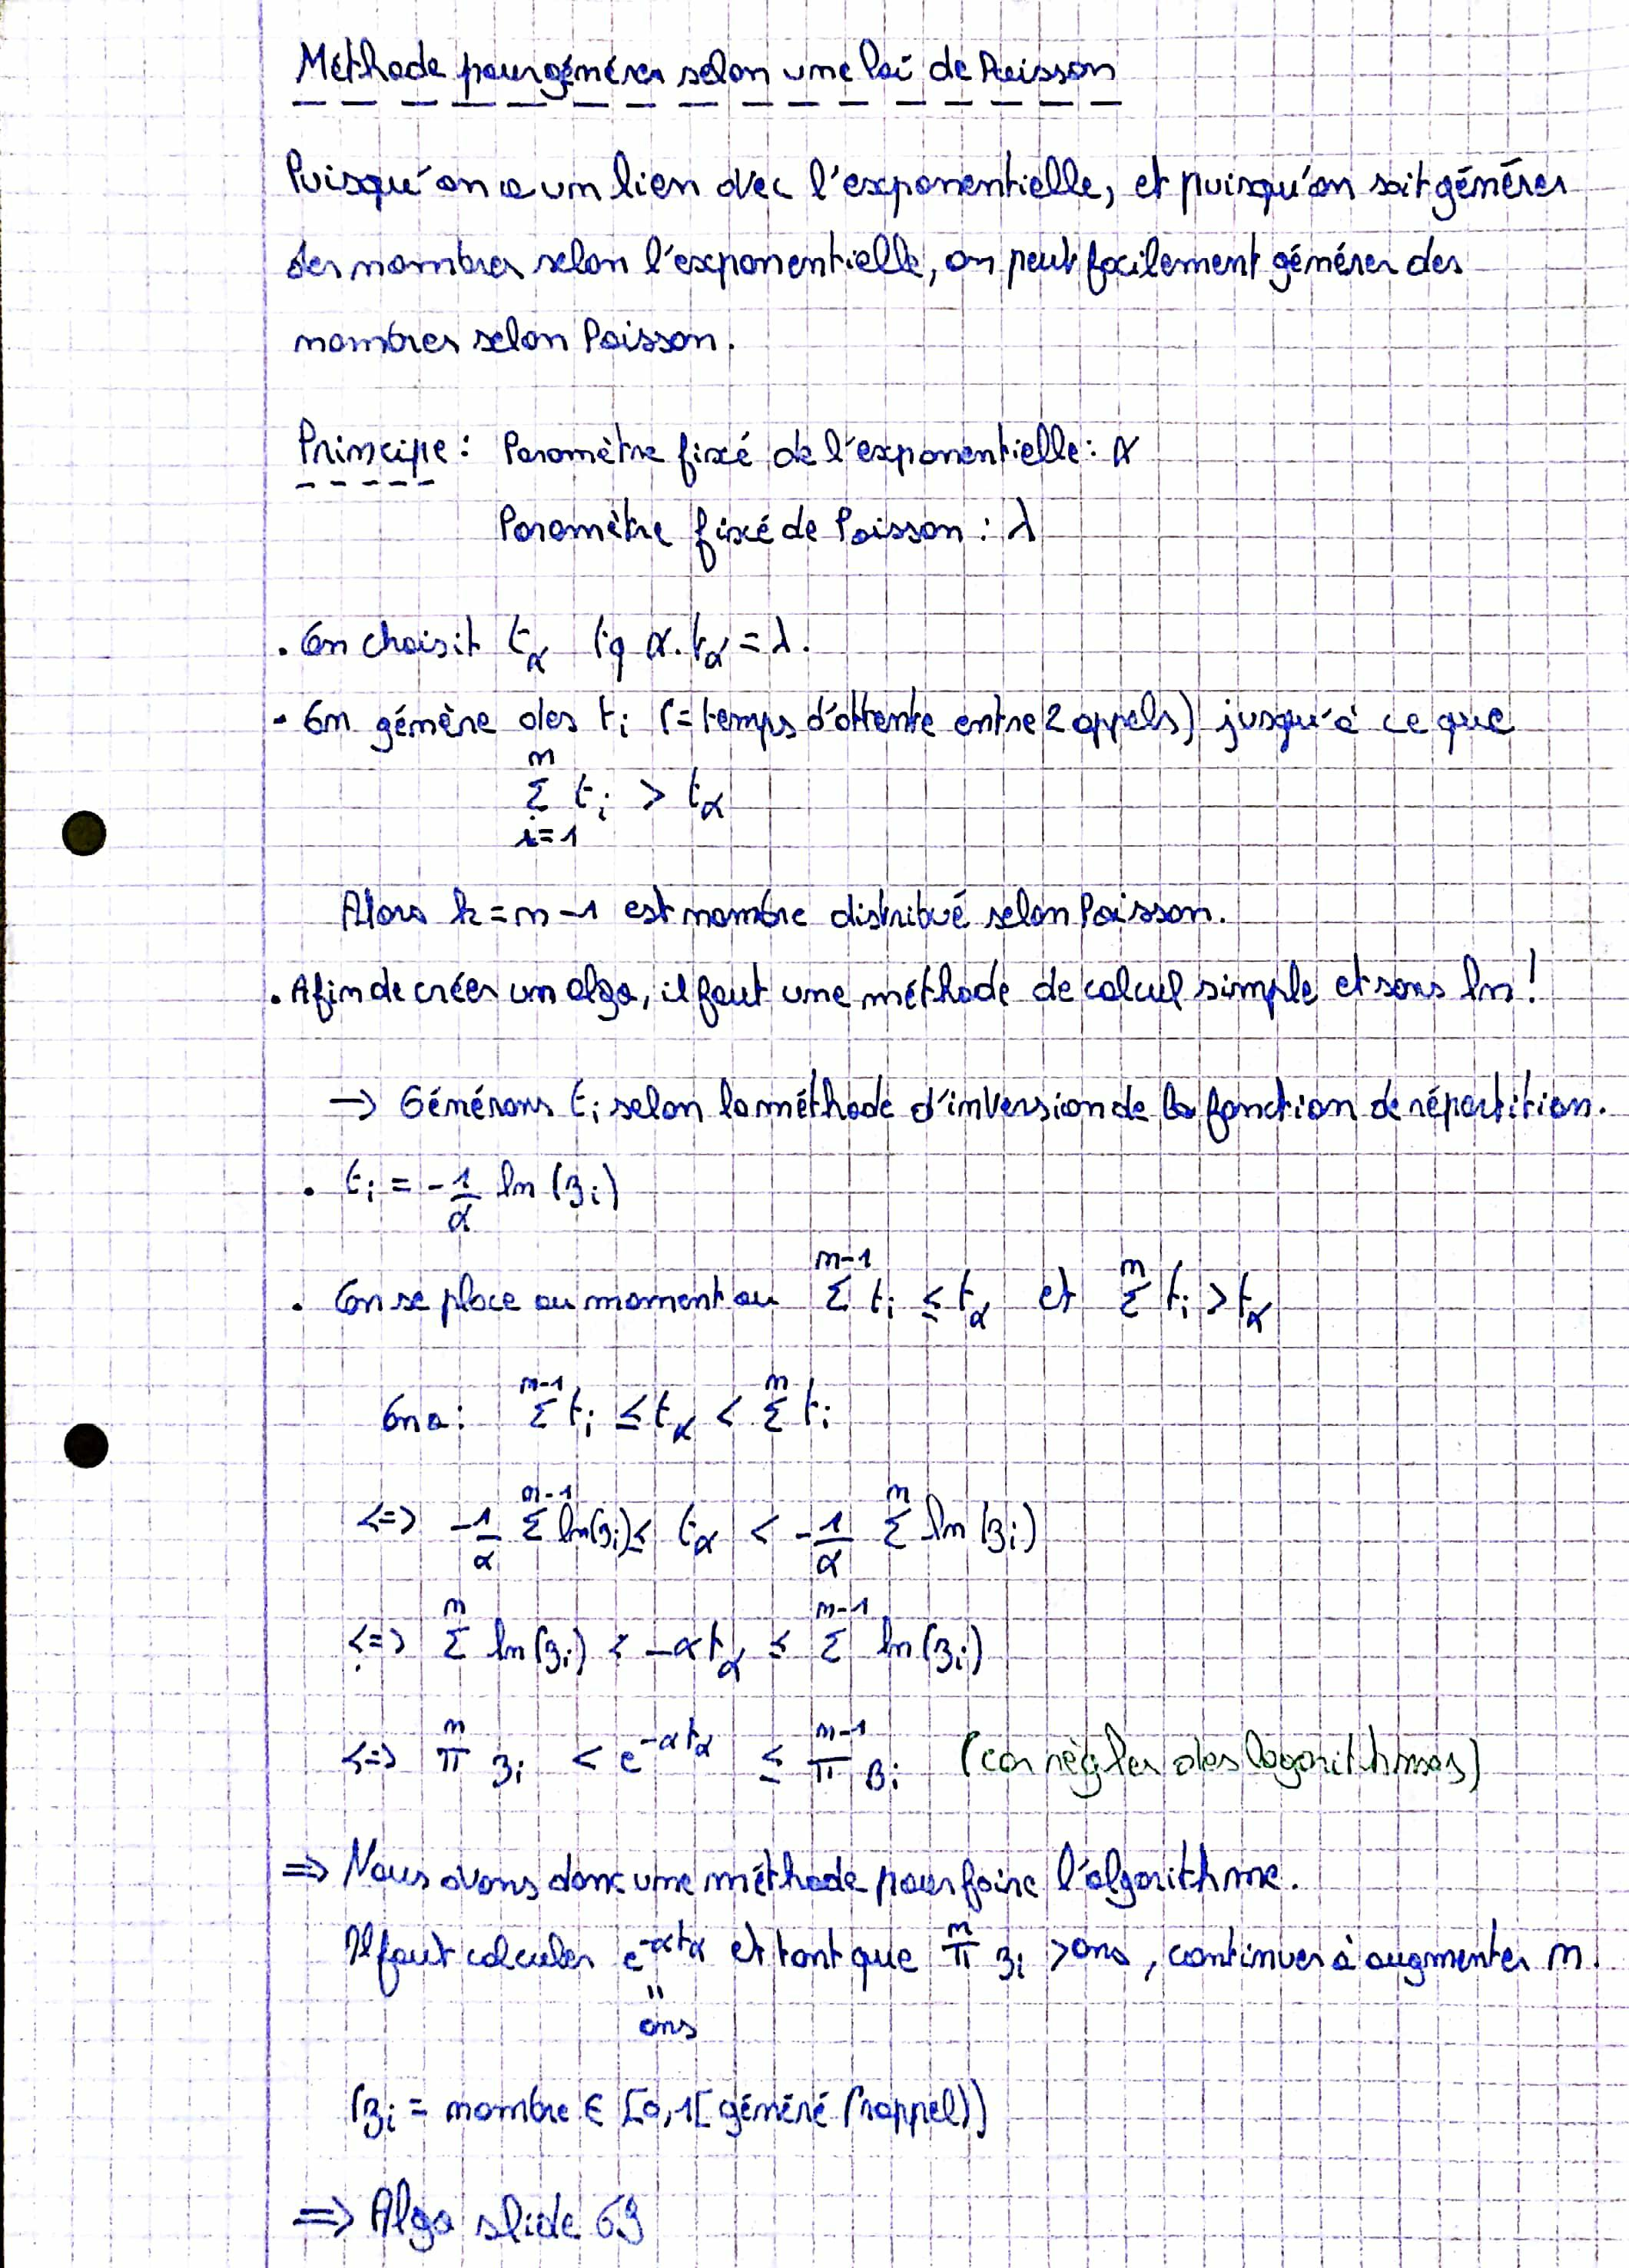
\includegraphics[width=\textwidth]{Jonathan(7)}
\end{figure}
\subsection{Loi normale - méthodes approchées}
\textbf{\underline{Méthode 1}}

Densité de probabilité de la loi normale centrée réduite: $$f(x)=\frac{1}{\sqrt{2\pi}}e^{-\frac{x^2}{2}}$$

Fonction de répartition de la loi normale centrée réduite: $$F(x)=P(X \leq x)=\frac{1}{\sqrt{2\pi}} \int_{-\infty}^{x} e^{-\frac{t^2}{2}} \, \mathrm dt$$

On pourrait utiliser la fonction réciproque de la fonction de répartition, $F^{-1}(x)$, pour générer des nombres suivant une loi normale centrée réduite. Cependant,
il n'existe pas d'expression analytique pour $F(x)$. De plus les résultats seraient insatisfaisants.
\vspace{0.3cm}

\textbf{\underline{Méthode 2}}

Soit $U_{1}, U_{2},...,U_{12}$ douze variables indépendantes de loi uniforme dans [0,1], alors $(\sum\limits_{i=1}^{12} U_{i})-6$ est de moyenne nulle et d'écart type unitaire.
Par le théorème de la limite centrale, cette variable suit approximativement une loi normale centrée réduite. Le résultat reste néanmoins toujours insatisfaisant.

Rappel théorème de la limite centrale: Soit une suite de v.a $X_1, X_2,..., X_n$ indépendantes et de même loi (donc de même moyenne $\mu$ et de même écart-type $\sigma$)
\[ Y_{n}=\frac{\sum\limits_{i=1}^{n} X_i -n\mu}{\sigma \sqrt{n}}\ \leadsto \ N(0,1)\text{ lorsque n tend vers }\infty \]
 
\subsection{Loi normale - méthode polaire}
La méthode de Box-Muller permet de générer des paires de nombres aléatoires suivant une distribution normale centrée réduite à partir
de nombres suivant une loi uniforme.

Soient $U_1$ et $U_2$ générés uniformément dans $[0, 1]$, alors
\[
		\begin{split}
		Z_1&=\sqrt{-2 \ln{U_1}}\cos(2\pi U_2) \leadsto N(0,1)\\
		Z_2&=\sqrt{-2 \ln{U_1}}\sin(2\pi U_2) \leadsto N(0,1)
		\end{split}
\]

Cet algorithme est simple à réaliser mais peu efficace étant donné les logarithmes, racines et fonctions trigonométriques.
\newpage

La forme polaire fût introduite plus tard pour combler ce manque de performance.
Cette forme s'appuie sur la méthode d'échantillonnage à rejet (=gaspillage de temps de calcul), cependant elle reste plus rapide.

Principe:
\begin{enumerate}
	\item Générer $U_1$ et $U_2$ uniformes dans $[0,1[$
	\item Soient $V_1=2U_1-1$ et $V_2=2U_2-1$ ($V_1$ et $V_2$ sont donc uniformes dans $[-1,1[$)
	\item Soit $S=V_1^2+V_2^2$
	\item Si $S>1$ alors on rejette $S$ et on recommence en 1.
	\item Sinon, on a
		\[
		\begin{split}
		X_1&=V_1\sqrt{-\frac{2\ln{S}}{S}} \leadsto N(0,1)\\
		X_2&=V_2\sqrt{-\frac{2\ln{S}}{S}} \leadsto N(0,1)
		\end{split}
		\]
\end{enumerate}
\vspace{0.3cm}
\begin{figure}[h]
   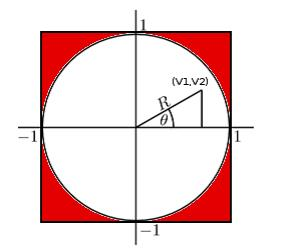
\includegraphics[width=6cm]{cercle}
	\centering
\end{figure}

Preuve:
A l'étape 4, Si $S<1$, le point $(V_1, V_2)$ est un point uniforme dans le cercle unité. Maintenant si on transforme en coordonnées polaires:
\[V_1 = R \cos{\Theta}\]
\[V_2 = R \sin{\Theta}\]

on trouve alors \[S = V_1^2+V_2^2 = R^2\]
\[X_1 = \sqrt{\frac{-2\ln{(S)}V_1^2}{S}} = \sqrt{\frac{-2\ln{(S)R^2\cos^2{\Theta}}}{R^2}} = \sqrt{-2\ln{S}}\cos{\Theta}\]
\[X_2 = \sqrt{\frac{-2\ln{(S)}V_2^2}{S}} = \sqrt{\frac{-2\ln{(S)R^2\sin^2{\Theta}}}{R^2}} = \sqrt{-2\ln{S}}\sin{\Theta}\]
\vspace{0.3cm}

On pose $R'=\sqrt{-2\ln{S}}$ et $\Theta' = \Theta$, on a donc $X_1=R'\cos{\Theta'}$ et $X_2=R'\sin{\Theta'}$. Il est évident que $R'$ et
$\Theta'$ sont indépendant car $R$ et $\Theta$ sont indépendants dans le cercle unité. Aussi, on a que 
\begin{itemize}
 \item $\Theta'$ est uniformément distribué entre 0 et $2\pi$
 \item $P(R'\leq r) = P(-2\ln(S)\leq r^2)$ = $P(S\geq e^{\frac{-r^2}{2}}) = 1-e^{\frac{-r^2}{2}}$ car $S=R^2$ est uniformément distribué entre
 0 et 1.
\end{itemize}

La probabilité que $R'$ se trouve entre $r$ et $r+dr$ est donc la dérivée de $1-e^{\frac{-r^2}{2}}$, à savoir $re^{\frac{-r^2}{2}}$.

De la même façon, la probabilité que $\Theta'$ se trouve entre $\theta$ et $\theta+d\theta$ est $(\frac{1}{2\pi})d\theta$.
\vspace{0.3cm}

La probabilité jointe que $X_1\leq x_1$ et $X_2\leq x_2$ peut maintenant être calculée de la façon suivante:

\begin{align}
 \int_{\{(r,\theta)|r \cos{\theta} \leq x_1, r\sin{\theta} \leq x_2\}} \frac{1}{2\pi}e^{-\frac{r^2}{2}}r\ dr\ d\theta
 & = \frac{1}{2\pi}\int_{\{(x,y)|x \leq x_1, y \leq x_2\}}e^{-(x^2+y^2)/2}dx\ dy \nonumber\\
 & = \left(\sqrt{\frac{1}{2\pi}} \int_{-\infty}^{x_1} e^{\frac{-x^2}{2}}dx \right)\left(\sqrt{\frac{1}{2\pi}} \int_{-\infty}^{x_2} e^{\frac{-y^2}{2}}dy \right) \nonumber
\end{align}
\vspace{0.3cm}

Ceci prouve que $X_1$ et $X_2$ sont indépendants et distribués selon une loi normale.

% Pages 138 à 139 du livre de référence (n° du lecteur PDF, pas des pages du livre)

\subsection{Méthode paire-impaire}
On veut tirer des nombres aléatoires selon une loi de la forme

\begin{equation}
    f(x) = 
        \begin{cases}
            Ce^{-h(x)} & \text{si } x \in [a, b] \\
            0 & \text{sinon}
        \end{cases}
\end{equation}

avec $\forall x \in [a, b], h(x) \in [0, 1]$.

Pour simuler cette loi, on va accepter un $X \in [a, b[$ avec une probabilité $e^{-h(x)}$ via l'algorithme suivant :

\begin{algorithm}[H]
    \caption{Méthode paire-impaire}
    \begin{algorithmic}[1]
        \Do
            \State Prenons $U$ tiré selon une loi uniforme sur $[0, 1[$
            \State $X \gets a + (b-a)\,U$ \Comment{$X$ est uniforme sur $[a, b[$}
            \State $V_0 \gets h(X)$
            \State $i \gets 0$
            \Do
                \State $i \gets i+1$
                \State Prenons $V_i$ tiré selon une loi uniforme sur $[0, 1[$
            \DoWhile{$V_{i-1} \geq V_i$}
        \DoWhile{$i$ est pair}
        \State Accepter $X$
    \end{algorithmic}
\end{algorithm}

Vérifions que cet algorithme respecte bien la condition d'accepter $X$ avec une probabilité $e^{-h(X)}$.

Remarquons que les $V_i$ sont indépendants et distribués uniformément.

La probabilité que l'algorithme s'arrête pour un $i$ quelconque est
\begin{equation}
    P(i) = P\{(V_0 \geq V_1 \geq \dots \geq V_{i-1}) \wedge (V_{i-1} < V_i)\}
    \label{paireimpaire:eq:probaI}
\end{equation}

Sans tenir compte de l'ordre, la probabilité que $V_0 \geq V_1 \wedge V_0 \geq V_2 \wedge \dots \wedge V_0 \geq V_{i-1}$ est $V_0^{i-1}$ \footnote{La probabilité que $a \leq b$ est $b$, donc que $a \leq b \wedge c \leq b$ est $b^2$, et ainsi de suite.}. Comme $V_0 = h(X)$ (par construction), $V_0^{i-1} = h(X)^{i-1}$. Dans notre cas, comme on veut $V_0 \geq V_1 \geq \dots \geq V_{i-1}$, il n'y a qu'un seul ordre possible. Donc,
$$P\{V_0 \geq V_1 \geq \dots \geq V_{i-1}\} = \frac{[h(X)]^{i-1}}{(i-1)!}$$

De la même façon, $P\{V_{i-1} < V_i\} = \frac{[h(X)]^i}{i!}$.

Donc, \eqref{paireimpaire:eq:probaI} devient
\begin{equation}
    P(i) = \frac{[h(X)]^{i-1}}{(i-1)!} - \frac{[h(X)]^i}{i!}
\end{equation}

On n'accepte que si $i$ est impair. La probabilité de s'arrêter à une valeur de $i$ impaire vaut
\begin{align*}
    \sum_{i=1,3,5,\dots}^\infty \frac{[h(X)]^{i-1}}{(i-1)!} - \frac{[h(X)]^i}{i!} & = \sum_{j=0}^\infty (-1)^j \frac{[h(X)]^j}{j!} & \text{en mettant $i-1$ et $i$ ensemble} \\
    & = \sum_{j=0}^\infty \frac{[-h(X)]^j}{j!}\\
    & = e^{-h(X)} & \text{par le développement de Taylor}
\end{align*}

Donc, on obtient que l'algorithme s'arrête pour un $i$ impair (en d'autres termes, qu'il accepte un nombre $X$) avec une probabilité $e^{-h(X)}$, comme voulu.

Analysons maintenant le nombre moyen de nombres à générer avant d'en accepter un. Pour un $k \geq 1$ fixé (avec une probabilité qu'on s'arrête à $k$ qui vaut $P(k)$), il faut générer $k$ nombres.
\begin{align*}
    \mean{k} = \sum_{k=1}^\infty kP(k) & = \sum_{k=1}^\infty k \left\{ \frac{[h(X)]^{k-1}}{(k-1)!} - \frac{[h(X)]^k}{k!} \right\} & \text{Définition de $P(k)$} \\
    & = \sum_{k=1}^\infty k\frac{[h(X)]^{k-1}}{(k-1)!} - \sum_{k=1}^\infty k \frac{[h(X)]^k}{k!} \\
    & = \sum_{k=0}^\infty (k+1)\frac{[h(X)]^k}{k!} - \sum_{k=1}^\infty k \frac{[h(X)]^k}{k!} & \text{On change $k=1$ en $k=0$} \\
    & = \sum_{k=0}^\infty k \frac{[h(X)]^k}{k!} + \sum_{k=0}^\infty \frac{[h(X)]^k}{k!} - \sum_{k=1}^\infty k \frac{[h(X)]^k}{k!} \\
    & = \sum_{k=0}^\infty \frac{[h(X)]^k}{k!} + \sum_{k=1}^\infty k\frac{[h(X)]^k}{k!} - \sum_{k=1}^\infty k\frac{[h(X)]^k}{k!} & \text{Pour $k=0$, $\forall R, kR = 0$}\\
    & = \sum_{k=0}^\infty \frac{[h(X)]^k}{k!} + 0 \\
    & = e^{h(X)} & \text{Par le développement de Taylor} \\
    & \leq e & \text{$h(X) \in [0, 1]$}
\end{align*}

En conclusion, on génère peu de nombres en moyenne. Cette méthode est donc plutôt efficace et ne demande pas de calculs complexes (logarithmes, racines carrées, etc.), même pour simuler la loi normale.

\subsubsection{Loi normale}
On va essayer de simuler la partie positive de la distribution $f(x) = \sqrt{\frac{2}{\pi}} e^{-\frac{x^2}{2}}$. On peut décider aléatoirement si on multiplie par $-1$ à la fin (avec un tirage pile ou face, par exemple).

On suppose qu'on travaille sur un ordinateur binaire avec $n + 1$ bits de précision. Cet algorithme demande une table de valeurs\footnote{La table avec les 30 premières valeurs se trouvent à la slide 76 du cours (et j'ajoute $a_0 = 0$)} $\forall j \in [1,n+1], d_j = a_j - a_{j-1}$, avec $a_j$ défini par :
$$\int_{a_j}^{+\infty} f(x)dx = \frac{1}{2^j}$$

Prenons $\forall a_j \leq t \leq a_{j+1}$, $h(t) = \frac{t^2 - a_j^2}{2}$ et vérifions que $h(t)$ est une fonction valide pour la méthode paire-impaire, c'est-à-dire que $\forall a_j \leq t \leq a_{j+1}, h(t) \in [0, 1]$. Il est trivial que $h(t) \geq 0$ avec $t \geq a_j$. On veut montrer que $h(t) \leq 1 \iff t^2-a_j^2 \leq 2 \iff a_{j+1}^2 - a_j^2 \leq 2$.

Prenons $m(x) = e^{\frac{x^2}{2}} \int_x^{+\infty} e^{-\frac{t^2}{2}} dt$. Comme $\int_x^{+\infty}e^{-\frac{t^2}{2}} dt$ n'est pas calculable, calculons plutôt

\begin{align*}
    \int_x^{+\infty} \frac{e^{-\frac{t^2}{2}}}{t^2} dt
    & = \left.- \frac{1}{t}e^{-\frac{t^2}{2}}\right]_x^{+\infty} - \int_x^{+\infty}\frac{-t e^{-\frac{t^2}{2}}}{-t} dt & \text{Intégration par partie} \\
    & = \frac{e^{-\frac{x^2}{2}}}{x} - \int_x^{+\infty}e^{-\frac{t^2}{2}} dt & \text{$e^{-\infty}=0$}\\
    e^{\frac{x^2}{2}} \int_x^{+\infty} \frac{e^{-\frac{t^2}{2}}}{t^2} dt & = \frac{1}{x} - m(x) & \text{On multiplie par $e^{\frac{x^2}{2}}$}
\end{align*}

Donc, on obtient que
$$m(x) = \frac{1}{x} - e^{\frac{x^2}{2}} \int_x^{+\infty}\frac{e^{-\frac{t^2}{2}}}{t^2} dt < \frac{1}{x}$$

Regardons la croissance de $m$ en dérivant $m(x) = e^\frac{x^2}{2}\int_x^{+\infty}e^{-\frac{t^2}{2}}dt$ :
\begin{align*}
    m'(x) & = x\ m(x) + e^\frac{x^2}{2} \left[ -e^{-\frac{t^2}{2}} \right]_{-\infty}^x \\
    & = x\ m(x) - 1 \\
    & < x\frac{1}{x} - 1 & \text{$m(x) < \frac{1}{x}$}\\
    & = 0
\end{align*}

Donc, $m$ est décroissante.

\newpage

Posons $y = \sqrt{x^2 + 2\,ln(2)}$, donc $y^2 = x^2 + 2\,ln(2)$ et $y > x \Rightarrow m(y) < m(x)$ (par décroissance).

\begin{align*}
    m(y) &= e^\frac{y^2}{2} \int_y^{+\infty}e^{-\frac{t^2}{2}} dt \\
    \iff \int_y^{+\infty}e^{-\frac{t^2}{2}} dt & = e^{-\frac{y^2}{2}} m(y) \\
    & = e^{\frac{-x^2 - 2\,ln(2)}{2}} m(y)\\
    & = \frac{1}{2} e^{-\frac{x^2}{2}}m(y) \\
    & < \frac{1}{2} e^{-\frac{x^2}{2}}m(x)
\end{align*}

Posons $x = a_j$ et multiplions les deux côtés par $\sqrt{\frac{2}{\pi}}$ :
\begin{align*}
    \sqrt{\frac{2}{\pi}}\,\int_y^{+\infty} e^{-\frac{t^2}{2}}dt & < \frac{1}{2}\sqrt{\frac{2}{\pi}}\,e^{-\frac{a_j^2}{2}} m(a_j)\\
    & = \frac{1}{2}\sqrt{\frac{2}{\pi}}\,e^{-\frac{a_j^2}{2}} e^\frac{a_j^2}{2}\int_{a_j}^{+\infty}e^{-\frac{t^2}{2}} dt & \text{Par définition de $m(x)$}\\
    & = \frac{1}{2} \frac{1}{2^j} & \text{Par définition des $a_j$} \\
    & = \frac{1}{2^{j+1}} \\
    & = \sqrt{\frac{2}{\pi}}\,\int_{a_{j+1}}^{+\infty} e^{-\frac{t^2}{2}} dt & \text{Par définition des $a_j$}
\end{align*}

On a $\sqrt{\frac{2}{\pi}}\,\int_y^{+\infty} e^{-\frac{t^2}{2}}dt < \sqrt{\frac{2}{\pi}}\,\int_{a_{j+1}}^{+\infty} e^{-\frac{t^2}{2}} dt$. La seule différence entre les deux termes est la borne inférieure de l'intégrale. Pour respecter l'inégalité, il faut que $y > a_{j+1}$ (si vous voyez l'intégrale comme une somme, on "retire" des termes pour avoir une somme plus petite).

Pour finir, on a :
\begin{align*}
    y & > a_{j+1}\\
    \implies \sqrt{a_j^2 + 2\,ln(2)} &> a_{j+1}\\
    \implies a_j^2+2\,ln(2) & > a_{j+1}^2\\
    \implies a_{j+1}^2 - a_j^2 &< 2\,ln(2)\\
    & < 2
\end{align*}

En conclusion, on a bien $a_{j+1}^2 - a_j^2\leq2$, donc $h(t)$ est une fonction valide pour la méthode paire-impaire pour la loi normale.

L'algorithme suivant est une version spécifique à la loi normale avec $h(t) = \frac{t^2-a^2}{2}$ de la méthode paire-impaire. On va calculer $h(x) = \frac{x^2-a^2}{2} = \frac{y^2 + a\,y}{2}$ en posant $y = x-a \iff x = y + a$. On va donc déterminer aléatoirement un $y$ (en respectant la probabilité de rejet).

\begin{algorithm}[H]
    \caption{Méthode paire-impaire pour la loi normale}
    \begin{algorithmic}[1]
        \State Générer avec une loi uniforme $U \gets (b_0, b_1, b_2, \dots, b_n)$ \Comment{Un nombre en binaire}
        \State $B \gets b_0$
        \State $j \gets 1$
        \State $a \gets 0$
        \While{$j < n+1 \wedge b_j=1$} \Comment{On détermine d'abord le $a$}
            \State $a \gets a + d_j$
            \State $j \gets j + 1$
        \EndWhile \Comment{On s'arrête en $j$ avec une probabilité $\frac{1}{2^j}$}
        \Do
            \State Générer avec une loi uniforme $Y \in [0, d_j[$ \Comment{On peut prendre $Y \gets d_j\,(b_{j+1}, \dots, b_n)$}
            \State $V \gets (\frac{1}{2}Y + a)Y$
            \Do
                \State Générer avec une loi uniforme $U \in [0, 1[$
            \DoWhile{$U = V$}
        \DoWhile{$U < V$} \Comment{Pour simuler le cas pair (rejet)}
        \State $X \gets a + Y$ \Comment{$X \in [a_{j-1}, a_j]$}
        \If{$B = 1$}
            \State $X \gets -X$
        \EndIf
    \end{algorithmic}
\end{algorithm}

% p.80-81 :
    % On veut simuler n'importe quelle loi de proba !
    % On va créer un rectangle dont le point en bas à gauche est (0, -v_max) et de taille (u, 2v_max)
    % Traçons le segment (0, 0) -- (u, v) et notons x son coefficient angulaire

    % On veut prouver que la courbe de formule u^2 = f(v/u) est bonne
    % On veut déterminer l'aire de la zone turquoise et l'aire de la zone colorée
    % En faisant le rapport entre les deux, on doit obtenir l'intégrale de -inf à x de f(t)dt
    % Intégrale de -inf à +inf de f(t)dt = 1 car loi de proba
    % dénominateur : tout le cercle ?
    % numérateur : la partie turquoise
    
% Notes diverses :
    % y = a*x+b : a = coefficient angulaire et b ordonnée à l'origine

% p 139-141

\subsection{Méthode de Kinderman et Monahan}
On cherche une méthode pour simuler n'importe quelle loi de probabilité $f(x)$.

On va prendre un rectangle dont le coin inférieur gauche se trouve en $(0, -u_{max})$ et de taille $(u_{max}, 2\,v_{max})$. On tire aléatoirement un point $(u, v$), on trace le segment $(0, 0) - (u, v)$ et on note $x$ le coefficient angulaire de ce segment.

Figure : cf cours p.80

A l'intérieur du rectangle, on définit une courbe telle qu'on rejette les points qui tombent en dehors. Sur la figure du cours, il s'agit du cercle mais ça peut être une autre courbe. On veut que les points acceptés soient tels que $x$ est distribué suivant la loi $f(x)$. On vérifie si le point $(u, v)$ est bien dans la courbe. Si oui, alors $x \gets \frac{v}{u}$.

\subsubsection{Courbe}
Pour être dans la courbe, les points $(u, v)$ doivent respecter la condition suivante.
\begin{equation}
    u > 0, u^2\leq f(\frac{v}{u})
    \label{eq:cercle}
\end{equation}

Montrons que la courbe voulue est définie par $u^2 = f(\frac{v}{u}) \iff u = \sqrt{f(\frac{v}{u})}$. Pour ce faire, on va déterminer l'aire sous la courbe et l'aire de la surface turquoise (sur le dessin) pour calculer leur rapport. Comme on veut que $x$ soit distribué selon la loi $f(x)$, le rapport doit être $\int_{-\infty}^x f(t)\,dt$.

\newpage

Calculons l'aire du "cercle" (sur le dessin), c'est-à-dire $\int_{\substack{u > 0\\u^2\leq f(\frac{v}{u})}} du\,dv$ (par \eqref{eq:cercle}). Soit $t = \frac{v}{u} \iff v = tu$, donc $dv = u\,dt$ :
\begin{align*}
    \int_{\substack{u > 0\\u^2 \leq f(t)}} u\,du\,dt &= \int_{-\infty}^{+\infty} dt \int_0^{\sqrt{f(t)}} u\,du & \text{Changement de variables, et donc, de bornes}\\
    & = \int_{-\infty}^{+\infty} dt \left. \frac{u^2}{2} \right ]_0^{\sqrt{f(t)}}\\
    & = \int_{-\infty}^{+\infty}dt \frac{f(t)}{2}\\
    & = \frac{1}{2} & \text{car on suppose que $f(x)$ est une loi de probabilité}
\end{align*}

Calculons maintenant l'aire de la surface turquoise (sur le dessin), c'est-à-dire qu'on rajoute la contrainte $\frac{v}{u} \leq x$, $\int_{\substack{u>0\\u^2\leq f(\frac{v}{u})\\\frac{v}{u}\leq x}} du\,dv$. Soit $t = \frac{v}{u} \iff v = u\,t$, donc $dv = u\, dt$ :
\begin{align*}
    \int_{-\infty}^xdt\ \int_0^{\sqrt{f(t)}} u\, du = \frac{1}{2} \int_{-\infty}^x f(t)\,dt
\end{align*}

Calculons maintenant le rapport entre la surface turquoise et toute la courbe :
$$ \frac{\frac{1}{2}\int_{-\infty}^x f(t)\,dt}{\frac{1}{2}} = \int_{-\infty}^x f(t)\,dt$$

On obtient bien $\int_{-\infty}^x f(t)\, dt$. Donc, la courbe voulue est bien définie par $u^2 = f(\frac{v}{u})$.

\subsubsection{Loi normale}
On veut simuler la fonction de probabilité $f(t) = e^{-\frac{t^2}{2}}$. Rappelons que $u^2 \leq f(\frac{v}{u})$. On obtient donc
\begin{align*}
    u^2 &\leq e^{-\frac{\frac{v^2}{u^2}}{2}}\\
    ln(u^2) &\leq -\frac{v^2}{2\,u^2}\\
    \frac{v^2}{u^2} &\leq -4\,ln(u)\stepcounter{equation}\tag{\theequation}\label{eq:vcarreucarre}\\
    \iff \frac{1}{4}\frac{v^2}{u^2} &\leq -ln(u) \stepcounter{equation}\tag{\theequation}\label{eq:quartvcarreucarre}\\
\end{align*}

Prenons $u_{max} = 1$. On veut déterminer $v_{max}$, c'est-à-dire la valeur maximale de la courbe en $y$. On va chercher les points où le contour de la courbe change de concavité, c'est-à-dire où la dérivée vaut $0$. Donc, l'inégalité devient une égalité (pour avoir uniquement le contour de la courbe) et on calcule la dérivée de $\frac{v^2}{u^2} = -4\,ln(u) \iff v^2 = -4\,u^2\,ln(u)$ :
\begin{align*}
    2\,v\frac{\partial v}{\partial u} = -8\,u\,ln(u) - 4\,\frac{u^2}{u} &= 0 & = 0\ \text{car on cherche un extremum}\\
    \iff -4u (2\,ln(u)+1) &= 0\\
    \iff -4u = 0 \vee ln(u) &= -\frac{1}{2} & \text{On rejette $u = 0$ car on veut une courbe (pas une ligne)}\\
    \iff u &= e^{-\frac{1}{2}}\\
\end{align*}

On a donc l'abscisse du point où la concavité de la courbe change. On va modifier \eqref{eq:vcarreucarre} en $v^2 \leq -4\,u^2\,ln(u)$ et appliquer $u=e^{-\frac{1}{2}}$.
\begin{align*}
    v_{max}^2 &= -4\,u^2\,ln(u)\\
    & = -4\,(e^{-\frac{1}{2}})^2\,ln(e^{-\frac{1}{2}})\\
    & = -4\,e^{-\frac{2}{2}}\,\frac{-1}{2} & \text{Propriétés des exposants et des $ln$}\\
    & = 2\,e^{-1}\\
    & = \frac{2}{e}\\
    \implies v_{max} &= \sqrt{\frac{2}{e}}
\end{align*}

Cette méthode appliquée telle quelle est lente. En effet, pour chaque $x$ à générer, il faut calculer un logarithme. On va donc encadrer la courbe préalablement définie par deux courbes plus simples. Si le point généré est entre ces deux courbes, alors on vérifiera plus précisement avec le logarithme. Si le point est dans la plus petite des deux, le point est directement accepté. S'il est hors de la plus grande, il est directement rejeté.

Déterminons ces deux courbes
\begin{align*}
    \forall x, e^x &\geq 1+x & \text{Par propriété de l'exponentielle}\\
    \implies \forall c, e^{-1+cu} &\geq cu\\
    \implies -1+cu &\geq ln(c)+ln(u) & \forall a,b,\ ln(ab) = ln(a)+ln(b)\\
    \implies -ln(u) &\geq ln(c)-cu+1\stepcounter{equation}\tag{\theequation}\label{lnu1}\\
    \forall c', e^{-1+\frac{1}{c'u}} &\geq \frac{1}{c'u}\\
    \implies -1 + \frac{1}{c'u} &\geq -ln(c')-ln(u)\\
    \implies ln(c') + \frac{1}{c'u} - 1 &\geq -ln(u)\stepcounter{equation}\tag{\theequation}\label{lnu2}\\
\end{align*}

En combinant \eqref{lnu1} et \eqref{lnu2}, on a :
\begin{equation}
    ln(c) - cu + 1 \leq -ln(u) \leq ln(c') + \frac{1}{c'u} - 1
    \label{eq:lnu}
\end{equation}

$ln(c) - cu + 1$ décrit la courbe la plus petite et $ln(c') + \frac{1}{c'u} - 1$ décrit la courbe la plus grande.

Donc, pour un point $(u, v)$, on en déduit que :
\begin{itemize}
    \item On accepte systématiquement le point si $\frac{1}{4}(\frac{v}{u})^2 \leq ln(c) - cu + 1$ ($\leq -\,ln(u)$ donc on a bien ce qu'on veut)
    \item On rejette systématiquement le point si $ln(c') + \frac{1}{c'u} - 1 \leq \frac{1}{4}(\frac{v}{u})^2$
\end{itemize}

Il y a encore des logarithmes MAIS on peut fixer les valeurs de $c$ et $c'$. Donc, les logarithmes deviennent des constantes et on est content.

Déterminons $c$ pour avoir une surface la plus grande possible ($c'$ pour la plus petite possible).

Commençons par $c$
\begin{align}
    (\frac{v}{u})^2 &\leq 4(1 + ln(c)) - 4\,c\,u & \text{Par la formule d'acceptance (cf ci-dessus)}\nonumber\\
    |v| &\leq |u|\sqrt{4(1+ln(c)) - 4\,c\,u} & \text{On prend la racine carrée}\nonumber\\
    &= u\sqrt{a-b\,u}   & a = 4(1+ln(c))\text{ et } b = 4c \label{eq:maxu}
\end{align}

On veut maximiser $u$ car on veut une courbe la plus grande possible. Par construction, la plus grande valeur possible pour $u$ demande d'avoir $v=0$. Donc, dans \eqref{eq:maxu}, on pose $|v|=0$ et on remplace l'inégalité par une égalité (pour avoir le contour) :
\begin{align*}
    0 &= u\sqrt{a-b\,u}\\
    \iff u = 0\ &\vee \sqrt{a-b\,u} = 0\\
    \iff u = 0\ &\vee a-b\,u = 0\\
    \iff u = 0\ &\vee u = \frac{a}{b}
\end{align*}

Donc, on prend $u = \frac{a}{b}$ comme valeur maximale pour $u$.

On veut maximiser $R = 2\int_0^{\frac{a}{b}}du\,\int_0^{u\sqrt{a-bu}} dv = 2\int_0^{\frac{a}{b}} \left. v\right]_0^{u\sqrt{a-bu}}\,du = 2\int_0^{\frac{a}{b}} u\sqrt{a-bu}\,du$.

Soit $t=\sqrt{a-bu} \iff u = \frac{a-t^2}{b}$. Donc, $-\frac{b}{2\sqrt{a-bu}} du = dt \implies du = -\frac{2}{b}t\,dt$ (on passe de l'autre côté et par définition de $t$).

\begin{align*}
    R &= -\frac{4}{b^2}\int_{\sqrt{a}}^0 t^2(a-t^2)dt & \text{Ne pas oublier le changement de bornes}\\
    &= -\frac{4a}{b^2}\int_{\sqrt{a}}^0 t^2\,dt + \frac{4}{b^2}\int_{\sqrt{a}}^0 t^4\,dt\\
    &= -\frac{4a}{b^2}\left[\frac{t^3}{3}\right]_{\sqrt{a}}^0 + \frac{4}{b^2}\left[\frac{t^5}{5}\right]_{\sqrt{a}}^0\\
    &= \frac{-4a}{b^2}\,.\,\frac{-a^\frac{3}{2}}{3} + \frac{4}{b^2}\,.\,\frac{a^{\frac{5}{2}}}{5}\\
    &= \frac{4a^{\frac{5}{2}}}{3b^2} - \frac{4a^{\frac{5}{2}}}{5b^2}\\
    &= \frac{8a^{\frac{5}{2}}}{15b^2}\\
    &= \frac{2\sqrt{2}}{15}\frac{(1+ln(c))^{\frac{5}{2}}}{c^2} & \text{On remplace $a$ et $b$ par leurs valeurs}\stepcounter{equation}\tag{\theequation}\label{eq:R}
\end{align*}

On veut donc maximiser \eqref{eq:R}. Calculons d'abord quelques dérivées
\begin{align*}
    ln(c)' &= \frac{1}{c}\\
    ((1+ln(c))^{\frac{5}{2}})' &= \frac{5}{2}\frac{1}{c}(1+ln(c))^{\frac{3}{2}}\\
    R' &= \frac{2\sqrt{2}}{15c^4}\left(\frac{5}{2}c(1+ln(c))^\frac{3}{2} - 2c(1+ln(c))^{\frac{5}{2}}\right)\\
    &= \frac{2\sqrt{2}(1+ln(c))^{\frac{3}{2}}}{15c^3}\left(\frac{5}{2} - 2(1+ln(c))\right)
\end{align*}

Trouvons les racines de $R'$.
\begin{align*}
    R'&=0\\
    \iff \frac{(1+ln(c))^{\frac{3}{2}}}{c^3} = 0 &\vee \frac{5}{2} - 2(1+ln(c)) = 0\\
    \iff (1+ln(c)) = 0 &\vee (1+ln(c)) = \frac{5}{4}
\end{align*}

$(1+ln(c))=0$ n'est pas un maximum car $R=0$ dans ce cas. Donc, $(1+ln(c)) = \frac{5}{4}$ est maximum.
\begin{align*}
    1+ln(c) &= \frac{5}{4}\\
    \implies ln(c) &= \frac{1}{4}\\
    \implies c &= e^{\frac{1}{4}}
\end{align*}

On a (enfin) la valeur optimale pour $c$.

Pour résumer, on accepte toujours un point $(u, v)$ quand $\left(\frac{v}{u}\right)^2 \leq 5 - 4\,u\,e^{\frac{1}{4}}$

Pour la valeur de $c'$\dots\ On ne peut pas calculer les intégrales de façon analytique. Grâce à des fous qui ont fait des tests, la valeur optimale pour $c'$ est approximativement $e^{\nombre{1.35}}$.

Pour résumer, on refuse toujours un point $(u, v)$ quand $\frac{4e^{-\nombre{1.35}}}{u} + \nombre{1.4} \leq \left(\frac{v}{u}\right)^2$

\subsection{Loi normale - Rectangles et coins}
Pour un très grand nombre de tirages aléatoires, la méthode Rectangle et coins ou \linebreak Rectangle-wedge-tail est encore plus rapide que la méthode polaire.

Pour cette méthode on n'utilise que la partie droite de la distribution:
\[f(x)=\sqrt{\frac{2}{\pi}}e^{-\frac{x^2}{2}}\]

Nous allons également considérer la distribution comme une somme pondérée de fonctions:
\[f(x)=p_1f_1(x)+p_2f_2(x)+...+p_nf_n(x) \qquad \sum\limits_{i=1}^{n} p_i=1\]

Certaines densités de fonction $f_j(x)$ peuvent être plus compliquées à calculer, on pourra donc leur attribuer un $p_j$ plus petit afin de rendre l'algorithme plus efficace.
A présent, divisons l'aire sous notre demi-courbe en, par exemple, 31 parts.

\begin{center}
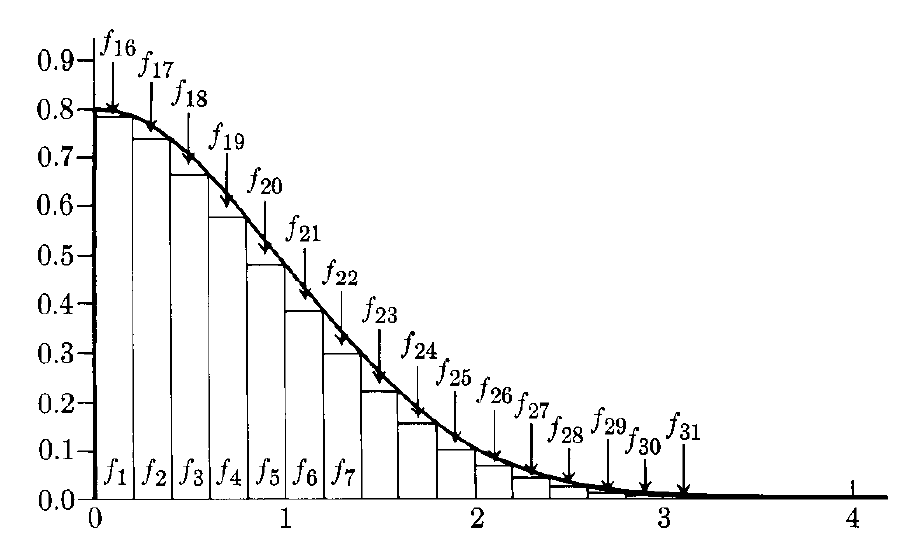
\includegraphics[width=10cm]{normal}
\end{center}

On remarque
\begin{itemize}
\item 15 rectangles représentant $p_1f_1(x),...,p_{15}f_{15}(x)$
\item 15 coins (au dessus des rectangles) représentant $p_{16}f_{16}(x),...,p_{30}f_{30}(x)$
\item 1 queue de la distribution représentant $p_{31}f_{31}(x)$
\end{itemize}

Les parties rectangulaires sont des distributions uniformes. Par exemple, $f_3(x)$ représente une variable aléatoire uniformément distribuée entre $\frac{2}{5}$ et $\frac{3}{5}$ (voir figure). L'aire du j-ième rectangle est
\[p_j=\frac{1}{5}f(\frac{j}{5})=\sqrt{\frac{2}{25\pi}}e^{-\frac{j^2}{50}} \qquad 1\leq j\leq 15\]
Dans ce cas on peut générer $U$ suivant une loi uniforme dans [0,1[ et prendre \[X=\frac{1}{5}U+S\qquad \text{où }S=\frac{j-1}{5}\text{ avec une probabilité }p_j\]

Notons que $p_1+p_2+...+p_{15}=0.9183$ et donc que cette zone représente près de 92\% de la génération. Pour les 8\% restant il faut générer une des distributions de \og coins\fg{}, $f_{16},...,f_{30}$.

On remarque que lorsque $x<1$ $(f_{16},...,f_{20})$, la concavité de la courbe est vers le bas tandis que si $x>1$ $(f_{21},...,f_{30})$, la concavité de la courbe est vers le haut.
Cependant la courbe est raisonnable et on peut l'encadrer entre deux droites parallèles comme montré ci-dessous.

\begin{center}
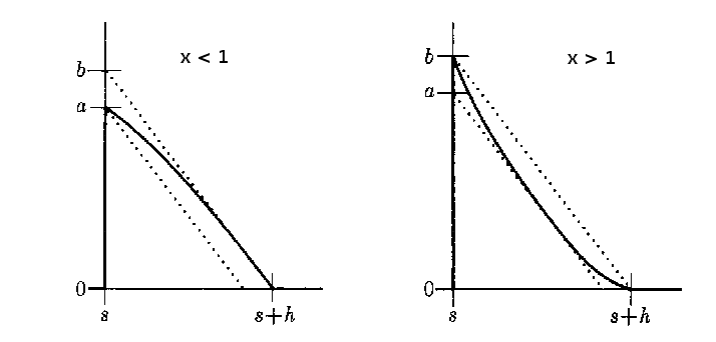
\includegraphics[width=12cm]{coins}
\end{center}

\begin{itemize}
	\item Pour $x<1$, on prend la tangente au point de droite et sa parallèle qui passe par l'autre point.
	\item Pour $x>1$, on joint les deux points extrêmes et on prend la tangente parallèle.
\end{itemize}

On obtient alors
\[
		\begin{aligned}
		a-\frac{b(x-s)}{h}&\leq& f(x) &\leq& b-\frac{b(x-s)}{h}\\
		\frac{a}{b} &\leq& \frac{1}{b}f(x)+\frac{(x-s)}{h} &\leq& 1
		\end{aligned}
\]

\begin{enumerate}
	\item On génère $U$ et $V$ uniformément dans [0, 1[ avec $V>U$ (sinon on échange)
	\item Si $V\leq \frac{a}{b}$, on va à l'étape 4.
	\item Si $V\leq U+(\frac{1}{b})f(s+hU)$, on retourne à l'étape 1. (si $\frac{a}{b}$ est proche de 1, on passera rarement dans ce cas)
	\item $X=s+hU$
\end{enumerate}

Vérification: voir cours, slide 90

Il ne nous reste plus qu'à traiter le cas de la queue de la distribution $f_{31}$. Ce cas ne se réalise qu'environ une fois sur 370.

\begin{itemize}
	\item Soit $f(x)$ une densité de probabilité suivant laquelle on génère des nombres aléatoires.
	\item Soit $g(x)$ une densité de probabilité suivant laquelle il est facile de générer des nombres aléatoires.
	\item Soit $f(x)\leq c\ g(x)$ où c est le plus petit possible $(c\geq 1)$
\end{itemize}

Algorithme pour générer des nombres selon $f(x)$:
\begin{enumerate}
	\item On génère $X$ selon $g(x)$.
	\item On génère $U$ uniforme dans [0,1[.
	\item Si $\frac{f(X)}{c\ g(X)}\leq U$ alors on retourne en 1 sinon on accepte X.
\end{enumerate}

La probabilité de rejeter X est alors
\[q=\int_{-\infty}^{+\infty} (g(t)dt\ (1-\frac{f(t)}{cg(t)}))=1-\frac{1}{c}\]

La probabilité d'accepter X est $\frac{1}{c}$

La probabilité d'accepter X généré suivant $g(x)$ (Point 3 de l'algo): $\frac{f(x)}{c*g(x)}$

La densité de probabilité de X: $f(x)=\frac{g(x)*\frac{f(x)}{c*g(x)}}{\frac{1}{c}}$

Prenons un exemple:\\
Soient
\[
f(t)=\frac{e^{-\frac{t^2}{2}}}{\int_3^{+\infty} e^{-\frac{u^2}{2}}du} \quad \text{et} \quad g(t)=a t e^{-\frac{t^2}{2}}
\]

On doit déterminer $a$ et $c$
\[
\int_3^{+\infty}g(t)dt=1=a\int_3^{+\infty}te^{-\frac{t^2}{2}}dt=\frac{a}{2}\int_9^{+\infty}e^{-\frac{t^2}{2}}dt^2=a\left [-e^{-\frac{x}{2}}\right ]_9^{+\infty}
\]

On tire donc que $a=e^{\frac{9}{2}}$, $g(t)=te^{\frac{9-t^2}{2}}$

La fonction de répartition de $g(x)$ notée $G(x)$:
\begin{align*}
G(x)=\int_3^xte^{\frac{9-t^2}{2}}dt &= \frac{1}{2}\int_9^{x^2}e^{\frac{9-t^2}{2}}dt^2\\
&= \frac{1}{2}e^{\frac{9}{2}}\int_9^{x^2}e^{-\frac{t^2}{2}}dt\\
&= e^{\frac{9}{2}}\left [-e^{-\frac{x^2}{2}}+e^{-\frac{9}{2}}\right ]\\
&= 1-e^{\frac{9-x^2}{2}}\\
&= y
\end{align*}

On peut alors générer $z=1-y=e^{\frac{9-x^2}{2}}$ dans $[0,1[$ et on trouve $x=\sqrt{9-2\ln{z}}$

Il nous manque encore $c$:
\begin{align*}
\frac{f(t)}{cg(t)} &=\frac{e^{-\frac{t^2}{2}}}{c\left [ \int_3^{+\infty} e^{-\frac{u^2}{2}}du\right ]te^{\frac{9-t^2}{2}}} \\
&=\frac{e^{-\frac{9}{2}}}{ct\int_3^{+\infty}e^{-\frac{u^2}{2}}du} \leq 1\\
&\Rightarrow c \geq \frac{e^{-\frac{9}{2}}}{t\int_3^{+\infty}e^{-\frac{u^2}{2}}du}
\end{align*}

On peut prendre $c=\frac{e^{-\frac{9}{2}}}{3\int_3^{+\infty}e^{-\frac{u^2}{2}}du}$

On accepte alors X si $U<\frac{F(X)}{cg(X)}=\frac{3}{X}$
\vspace{0.3cm}

\begin{figure}[h]
	\centering
  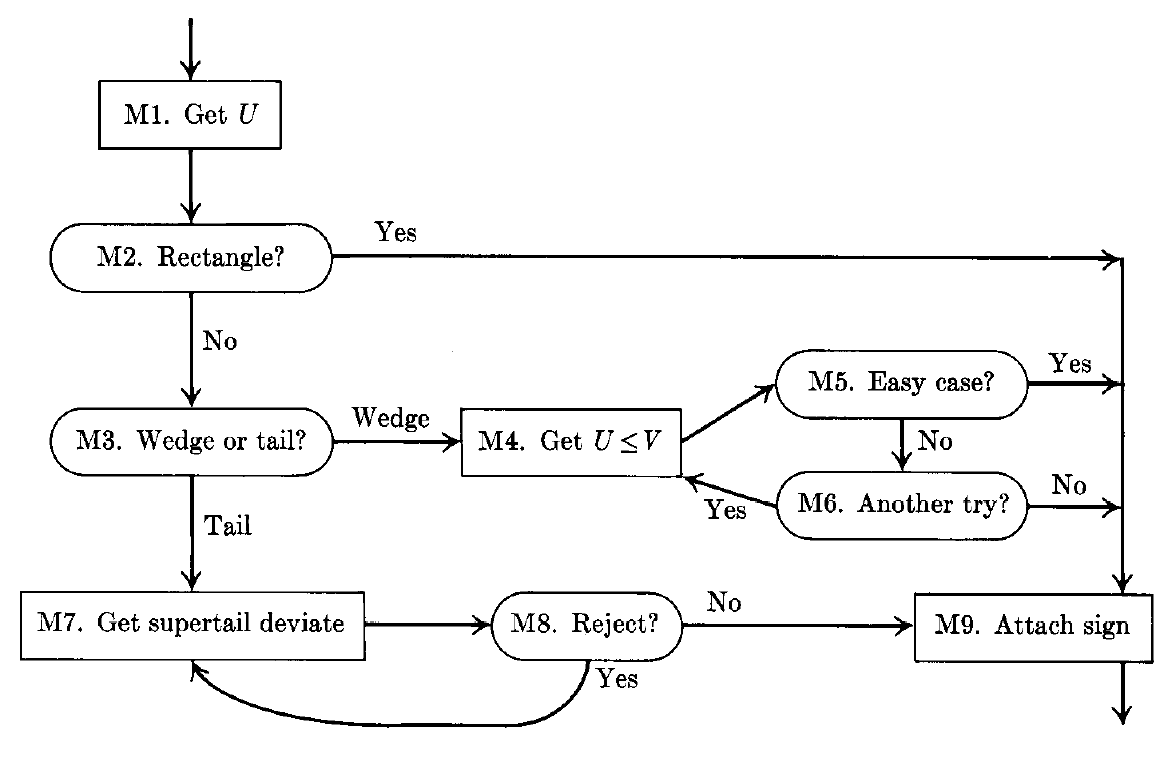
\includegraphics[width=12cm]{graphe}
	\caption{L'algorithme en résumé}
\end{figure}
\subsection{Loi exponentielle - minimisation aléatoire}
Cette méthode a pour but de générer des nombres pseudos aléatoires selon une loi exponentielle de la forme :
\begin{equation}
f(x) = 
\left\lbrace
	\begin{array}{ccc}
   	 1 - e^{-\lambda x} & \text{si x $\geq$ 0}\\ 
   	 0 & \text{sinon}
    \end{array}\right.
\end{equation}
\smallbreak
Nous avons déjà vu une méthode permettant de faire ça, mais nous devions calculer un logarithme, ce que nous voulons éviter. C'est pour cela que nous avons mis cette méthode en place.\\ \smallbreak
Soit $Q[k] = \frac{ln 2}{1!} + \frac{(ln 2)^2}{2!} + \frac{(ln 2)^3}{3!} + ... + \frac{(ln 2)^k}{k!}$\\ \smallbreak
On voit que $ Q[k] \rightarrow 1$ quand $k \rightarrow +\infty$. En effet, Q[k] représente le développement de Taylor sans le premier terme ($ + 1$) de $e^{ln(2)} = 2$. On a donc que ça tend vers $2 - 1 = 1$.\\ \smallbreak
En pratique on s'arrête quand $Q[k] > 1 -2^{1-n}$ pour des mots de n bits.\\ \smallbreak
\begin{algorithm}[H]
	\caption{Algorithme minimisation aléatoire}
	\begin{algorithmic}[1]
		\State Générer un nombre aléatoire suivant la loi uniforme $V = (b_{0}, b_{1}, ..., b_{n})$ (en binaire). Soit j le premier bit étant 1 ($P\{j = J\} = \frac{1}{2^{J+1}}$). Alors, soit $U = (b_{j+1},...,b_{n})$.\smallbreak
		\State Si $U < ln(2)$, alors $X \leftarrow \mu (j\,ln(2) + U)$ et on arrête l'algorithme ici.\smallbreak
		\State Trouver la plus petite valeur de k telle que $Q[k] > U$, générer k nombres aléatoires $U_{1}, U_{2}, ..., U_{k}$ . $V \leftarrow min(U_{1}, U_{2}, ..., U_{k})$\smallbreak
		\State Prendre $X \leftarrow \mu (j + V)\,ln(2)$
	\end{algorithmic}
\end{algorithm} 

L'algorithme est très facile à appliquer. Il faut juste comprendre pourquoi on obtient bien un nombre suivant une loi exponentielle.\\
Calculons la fonction de répartition de X et regardons si nous obtenons bien la fonction de répartition de la loi exponentielle ($1 - e^{-\lambda x}$).\\
\begin{equation}
\begin{split}
	P\{X \leq X_0\} =& (ln(2))\,P\left\{\mu(j\,ln(2) + U) \leq X_0\right\} +\\
	& \sum_{k=2}^{+\infty}\frac{(ln(2))^k}{k!}\,P\left\{\mu(j + V)\,ln(2) \leq X_0\right\}
\end{split}
\end{equation}
\smallbreak
La première ligne provient de la 2\ieme ligne de l'algorithme et la seconde provient de la $4^{eme}$ ligne de l'algorithme.
\paragraph{1ère ligne du calcul}
\begin{itemize}
\item ln(2) s'explique car on a $U<ln(2)$ (probabilité qu'un truc uniforme < X = X)
\item Le reste exprime juste $P\{X \leq X_0\}$ dans le cas où on est dans la seconde ligne de l'algo.
\end{itemize}
\paragraph{2ème ligne du calcul}
\begin{itemize}
\item La somme exprime les $U<Q[k]$ par le même raisonnement qu'au-dessus (probabilité qu'un truc uniforme < X = X), et vu qu'on a plusieurs k tq $U<Q[k]$, on obtient une somme sur les Q[k]. On commence cette somme à 2 puisque le cas $k=1$ est impossible puisque $U > ln(2)$ dans ce cas-ci.
\item Encore une fois, le reste exprime juste $P\{X \leq X_0\}$ dans le cas où on est dans la quatrième ligne de l'algo.
\end{itemize}
\smallbreak
Suite du calcul : \\ 
\begin{equation}
\begin{split}
=& (ln(2))\,P\left\{j + \frac{U}{ln(2)} \leq \frac{X_0}{\mu\,ln(2)}\right\} +\\
	& \sum_{k=2}^{+\infty}\frac{(ln(2))^k}{k!}\,P\left\{(j + V) \leq \frac{X_0}{\mu\,ln(2)}\right\}
\end{split}
\end{equation}

\begin{figure}[H]
    \includegraphics[width=\textwidth]{Dorian1}
\end{figure}
\begin{figure}[H]
    \includegraphics[width=\textwidth]{Dorian2}
\end{figure}
\begin{figure}[H]
    \includegraphics[width=\textwidth]{Dorian3}
\end{figure}
\begin{figure}[H]
    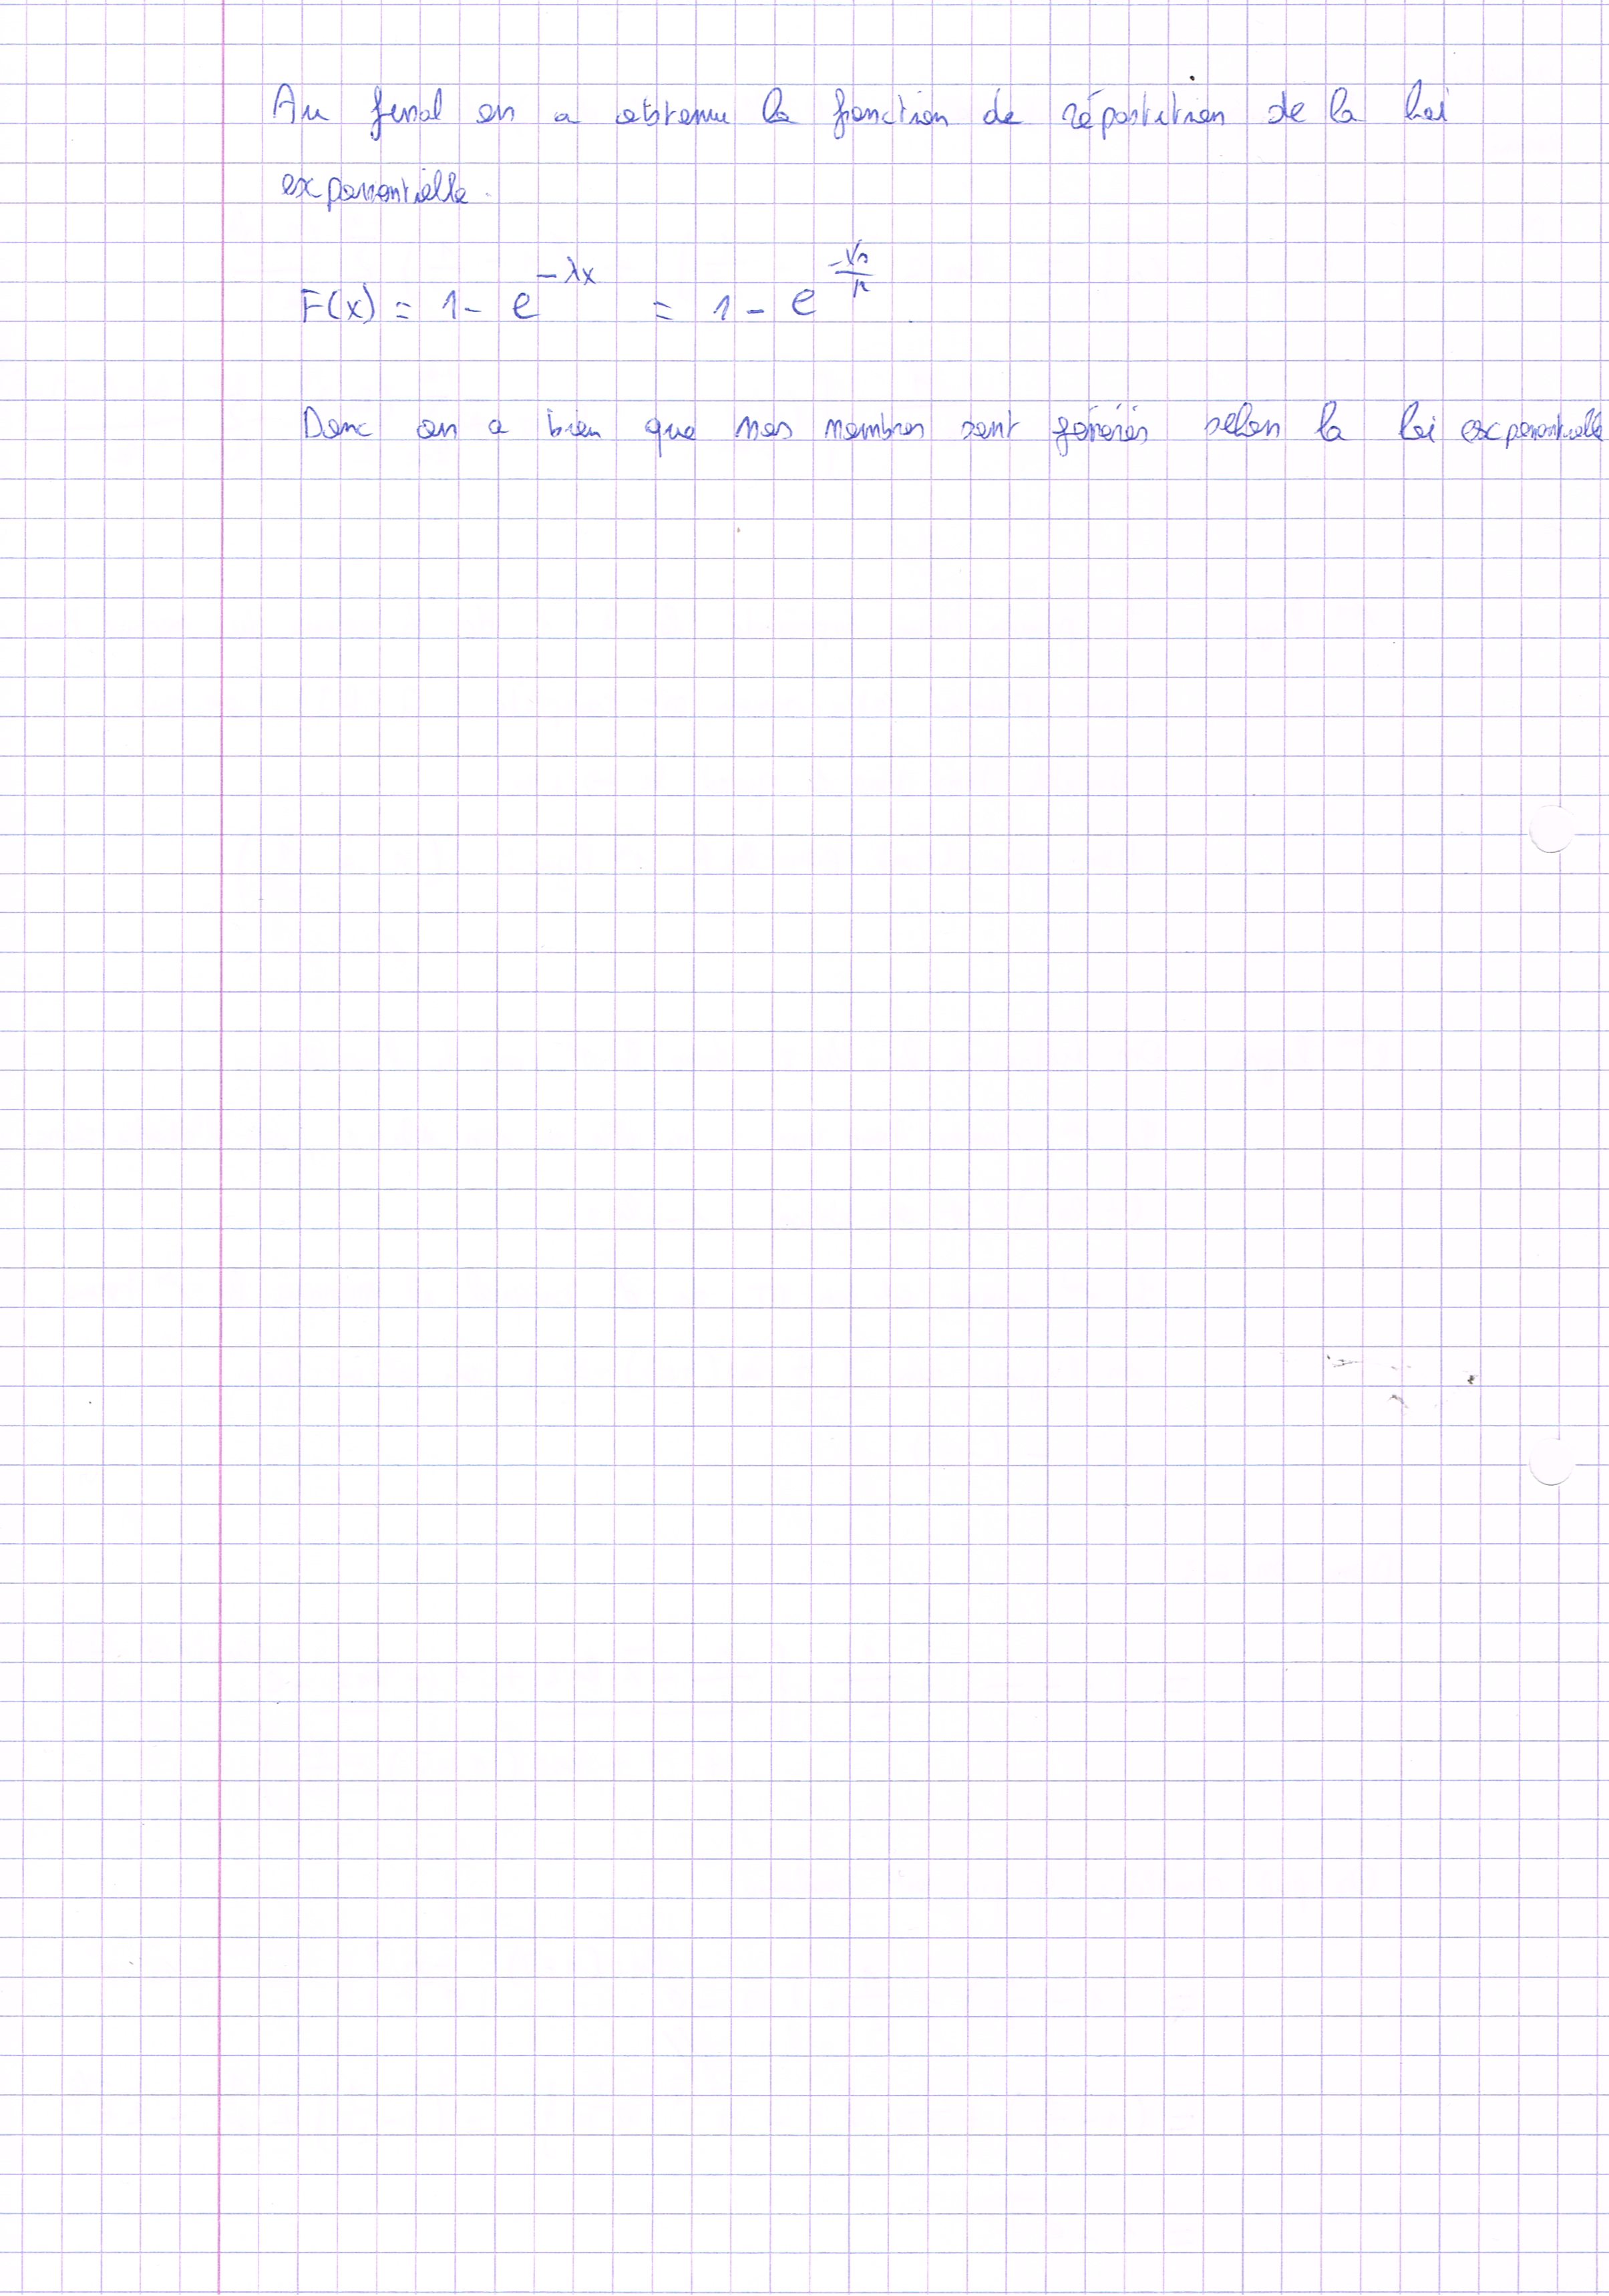
\includegraphics[width=\textwidth]{Dorian4}
\end{figure}

\end{document}
